\documentclass[twoside,12pt]{wipb}

\usepackage{blindtext}
\usepackage{enumitem}
\usepackage{xcolor}
\usepackage{amssymb}


\katedra{Nazwa katedry}
\typpracy{in�ynierska}
%typpracy{magisterska}
\temat{Temat pracy in�ynierskiej / magisterskiej.}
\autor{Gal Anonim}
\promotor{dr in�. Doktor In�ynier}
\indeks{12345}
\studia{stacjonarne}
\rokakademicki{2013/2014}
\profil{studia II stopnia}
\kierunekstudiow{informatyka}
\specjalnosc{In�ynieria Oprogramowania}
\zakres{1. Zakres 1\newline 2. Zakres 2\newline 3. Zakres 3}

\hypersetup{
pdfauthor={Gal Anonim},
pdftitle={Praca in�ynierska},
pdfsubject={Temat pracy},
pdfkeywords={praca magisterska jakie� inne s�owa kluczowe},
pdfpagemode=UseNone,
linkcolor=black,
citecolor=black,
urlcolor=black
} 

\setlength{\epigraphwidth}{1\textwidth}

\begin{document}

\maketitle

\chapter*{\centering{\vspace{1in}Summary}}
\addcontentsline{toc}{chapter}{Streszczenie}
 
\epigraphhead[40]{
Subject of diploma thesis

Temat po angielsku.}

Streszczenie pracy po angielsku.


\cleardoublepage
{\setstretch{1.0}

{\hfill Za��cznik nr 4 do �Zasad post�powania przy przygotowaniu i obronie\par }
{\hfill pracy dyplomowej na PB�\par }

\hfill Bia�ystok, dnia 05.01.2020 r.
\\*

\noindent \textbf{Gal Anonim}

\noindent Imiona i nazwisko studenta

\noindent \textbf{12345}

\noindent Nr albumu

\noindent \textbf{informatyka, stacjonarne}

\noindent Kierunek i forma studi�w

\noindent \textbf{dr in�. Doktor In�ynier}

\noindent Promotor pracy dyplomowej
\\*
\\*

{\centering \textbf{O�WIADCZENIE}\par }


Przedk�adaj�c w roku akademickim 2019/2020 Promotorowi \textbf{dr in�. Doktor In�ynier} prac� dyplomow� pt.: \textbf{Temat pracy}, dalej zwan� prac� dyplomow�, \textbf{o�wiadczam, �e}: 

\begin{enumerate}
\setlength\itemsep{0em}
\item[1)] praca dyplomowa stanowi wynik samodzielnej pracy tw�rczej; 
\item[2)] wykorzystuj�c w pracy dyplomowej materia�y �r�d�owe, w tym w szczeg�lno�ci: monografie, artyku�y naukowe, zestawienia zawieraj�ce wyniki bada� (opublikowane, jak i nieopublikowane), materia�y ze stron internetowych, w przypisach wskazywa�em/am ich autora, tytu�, miejsce i rok publikacji oraz stron�, z kt�rej pochodz� powo�ywane fragmenty, ponadto w pracy dyplomowej zamie�ci�em/am bibliografi�;
\item[3)] praca dyplomowa nie zawiera �adnych danych, informacji i materia��w, kt�rych publikacja nie jest prawnie dozwolona;
\item[4)] praca dyplomowa dotychczas nie stanowi�a podstawy nadania tytu�u zawodowego, stopnia naukowego, tytu�u naukowego oraz uzyskania innych kwalifikacji;
\item[5)] tre�� pracy dyplomowej przekazanej do dziekanatu Wydzia�u Informatyki jest jednakowa w wersji drukowanej oraz w formie elektronicznej;
\item[6)] jestem �wiadomy/a, �e naruszenie praw autorskich podlega odpowiedzialno�ci na podstawie przepis�w ustawy z dnia 4 lutego 1994 r. o prawie autorskim i prawach pokrewnych (Dz. U. z 2019 r. poz. 1231, p�n. zm.), jednocze�nie na podstawie przepis�w ustawy z dnia 20 lipca 2018 roku Prawo o szkolnictwie wy�szym i nauce (Dz. U. poz. 1668, z p�n. zm.) stanowi przes�ank� wszcz�cia post�powania dyscyplinarnego oraz stwierdzenia niewa�no�ci post�powania w sprawie nadania tytu�u zawodowego;
\item[7)] udzielam Politechnice Bia�ostockiej nieodp�atnej, nieograniczonej terytorialnie i czasowo licencji wy��cznej na umieszczenie i przechowywanie elektronicznej wersji pracy dyplomowej w zbiorach systemu Archiwum Prac Dyplomowych Politechniki Bia�ostockiej oraz jej zwielokrotniania i udost�pniania w formie elektronicznej w zakresie koniecznym do weryfikacji autorstwa tej pracy i ochrony przed przyw�aszczeniem jej autorstwa.  
\end{enumerate}
 
\hfill .���������������.
\begin{flushright}
czytelny podpis studenta	
\end{flushright}
}          


%\biblioteka{}

\pagestyle{plain}

\setcounter{tocdepth}{1}
\tableofcontents

\chapter*{Wst�p}
\addcontentsline{toc}{chapter}{Wst�p}
  
	Odpady generowane przez mieszka�c�w s� jednym z problem�w z jakimi w�adze musz� sobie radzi� w Polsce. Nie jest to problem jedynie wielkich metropolii ale r�wnie� mniejszych miasteczek. Ilo�� produkowanych �mieci jest olbrzymia, a to r�wnie� powoduje kolejne problemy. Segregacja oraz sk�adowanie to nie jest jedyny problem z jakim mo�na si� spotka�. Kolejnym utrudnieniem jakie mo�na wyr�ni� jest ich transport.

	W 2018 roku w Bia�ymstoku zosta� zorganizowany 24-godzinny Hackaton Miejski w Bia�ostockim Parku Naukowo-Technologicznym. Organizatorzy tego przedsi�wzi�cia przygotowali du�� ilo�� merytorycznych materia��w na temat zbi�rki odpad�w komunalnych w mie�cie Bia�ystok. Uczestnicy hackatonu zauwa�yli wiele problem�w z jakimi boryka si� miasto. Jednak najwi�ksz� uwag� organizator�w przyku�y inne anomalie.
	
	Jedna z grup zauwa�y�a, �e trasy jakie pokonuj� ci�ar�wki s� nieoptymalne. Jako przyk�ad zosta�a przedstawiona droga losowej ci�ar�wki. Mo�na by�o zauwa�y�, �e przebyta �cie�ka przecina si� w wielu miejscach. Na podstawie tylko jednego przyk�adu mo�na doj�� do wniosku, �e problem jest globalny i mo�e dotyczy� wszystkich tras. Organizatorzy przedsi�wzi�cia przyznali, �e nie przyk�adali do tego aspektu uwagi ale mo�e to by� kluczowe w oszcz�dno�ci czasu oraz pieni�dzy.
	
	Przy pomocy komputer�w oraz odpowiednio napisanego programu mo�na wyznaczy� �cie�ki kt�re b�d� spe�nia� za�o�enia biznesowe oraz b�d� odpowiednio optymalne. Wyzwaniem jest jedynie znalezienie odpowiedniego rozwi�zania kt�re nada prawid�owy kierunek przeprowadzanym optymalizacjom. Na przestrzeni lat zosta�o opracowanych wiele rozwi�za�. Niestety nie ka�de rozwi�zanie jest w stanie poradzi� sobie z konkretnymi danymi w ten sam spos�b.
	
	W naszej pracy magisterskiej wykorzystamy algorytmy dla kt�rych znajdziemy takie parametry wej�ciowe aby wynik ich prac by� jak najbardziej optymalny. Jako pierwsze rozwi�zanie zostanie przedstawiony algorytm genetyczny kt�ry zosta� opracowany przez Paw�a Stypu�kowskiego. Kamil ��towski przygotowa� i opisa� zagadnienia zwi�zane z algorytmem mr�wkowym. Na samym ko�cu kilka rozwi�za� heurystycznych zosta�o om�wionych przez Przemys�awa Noskowicza.
	
\chapter{Og�lny problem}

Problem komiwoja�era (ang. travelling salesman problem - TSP) nale�y do rodziny problem�w NP-trudnych. Znalezienie najlepszego rozwi�zania dla tego problemu jest trudne i fascynuje naukowc�w od wielu lat. Niekt�rzy poddaj� pod w�tpliwo�� znalezienie efektywnego rozwi�zania czyli takiego kt�rego czas dzia�ania jest maksymalnie wielomianowy. Aktualnie istnieje wiele rozwi�za� tego problemu, a proponowane podej�cia s� bardzo interesuj�ce. Niekt�re z nich bazuj� na lokalnych przeszukiwaniach grafu, a inne opieraj� si� na rozwoju.

Podobnym problemem do TSP jest problem konika szachowego. Problem ten jest problemem NP-zupe�nym. Ju� w XVIII wieku badania nad tym problemem rozpocz�� Euler. Rozwi�zanie tego problemu polega na znalezieniu �cie�ki jak� ma przeby� konik szachowy, tak aby odwiedzi� ka�de pole na szachownicy tylko i wy��cznie raz. Skoczek porusza si� po planszy zgodnie z okre�lonym ruchem, a plansza szachowa mo�e mie� r�ny rozmiar. Konik porusza si� a� do momentu odwiedzenia wszystkich p�l lub do momentu w kt�rym nie ma mo�liwo�ci odwiedzenia kolejnego pola.

Optymalizacja tras od zawsze jest obecna w historii ludzko�ci. Nawet takie trywialne problemy jak podr� pomi�dzy 3 miejscowo�ciami mo�e zosta� sklasyfikowany jako problem komiwoja�era. Chocia� dok�adne wskazanie na �r�d�o problemu TSP nie jest znane, to ju� w 1832 roku w przewodniku dla podr�uj�cych po Niemczech i Szwajcarii zosta�a zawarta informacja o optymalizacji trasy przejazdu. Nie ma tam zawartych �adnych teorii matematycznych w zwi�zku z czym nie mo�na uzna� tego dzie�a za pocz�tek rozwa�a� nad problemem komiwoja�era.

W XIX wieku William Hamilton stworzy� fundamenty pod definicj� TSP. W rozwi�zaniu problemu komiwoja�era nale�y znale�� cykl w grafie. W sk�ad takiego cyklu musi zosta� zawarty ka�dy z wierzcho�k�w. Ka�dy z wierzcho�k�w mo�e znajdowa� si� w rozwi�zaniu dok�adnie tylko raz. Cykl kt�ry spe�nia wymieniony warunek jest cyklem Hamiltona. Je�li w grafie mo�na wyr�ni� cykl z opisanymi powy�ej warunkami, to graf jest grafem Hamiltonowskim. 

Na \ref{kl_graf_nie_hamiltona} zosta� przedstawiony graf bez cyklu Hamiltona. W grafie tym nie mo�na znale�� takiego po��czenia kt�re zawiera wszystkie wierzcho�ki przechodz�c przez ka�dy z nich dok�adnie raz. Istnieje mo�liwo�� przej�cia przez wszystkie wierzcho�ki jedynie po powt�rnym odwiedzeniu przynajmniej jednego wierzcho�ka.

\begin{figure}[h]
	\centering
	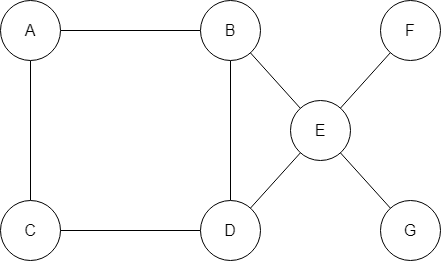
\includegraphics[scale=0.75]{grafika/kl_graf_nie_hamiltona.png}
	\caption{Graf bez cyklu Hamiltona.}
	\label{kl_graf_nie_hamiltona}
\end{figure}

Graf z \ref{kl_graf_hamiltona} posiada po��czenie kraw�dzi dzi�ki kt�remu mo�na przej�� po wszystkich wierzcho�kach dok�adnie raz. Takie przej�cie jest w�a�nie cyklem Hamiltona w zwi�zku z czym graf jest Hamiltonowski. Wyruszaj�c przyk�adowo z punktu F mo�emy przej�� kolejno do E - G - D - B - A - C. W ten spos�b odwiedzimy wszystkie wierzcho�ki tylko raz. 

\begin{figure}[h]
	\centering
	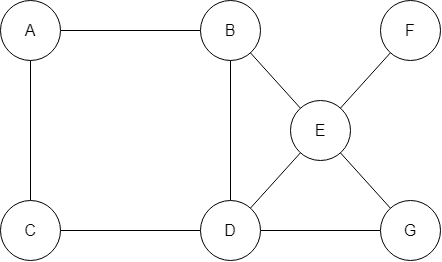
\includegraphics[scale=0.75]{grafika/kl_graf_hamiltona.png}
	\caption{Graf z cyklem Hamiltona.}
	\label{kl_graf_hamiltona}
\end{figure}

W latach 30 XX wieku Merrill Meeks Flood rozpocz�� rozwa�ania nad optymalizacj� przejazdu autobus�w szkolnych. Dzia�alno�� t� mo�emy uzna� za pocz�tek pracy nad problemem TSP. Wraz z up�ywem czasu zainteresowanie problemem optymalizacyjnym narasta�o a co za tym idzie powstawa�y nowe pomys�y na algorytmy. Jednak �aden z pomys��w nie jest w stanie zaproponowa� dok�adnego rozwi�zania kt�re jest w stanie przedstawi� rezultat w czasie wyra�onym za pomoc� wielomianu.

Jednym z proponowanych rozwi�za� jest algorytm Helda Karpa kt�ry jest oparty na programowaniu dynamicznym. Z�o�ono�� pami�ciowa tego algorytmy wynosi O(n razy 2 do n), a czasowa O(n do 2 razy 2 do n). W algorytmie tym na ka�dym kroku wyznaczamy punkt kt�ry powinien by� przedostatni na trasie. Aby wyznaczy� poprzednika nale�y skorzysta� ze wzoru w kt�rym poszukiwana jest najmniejsza warto�� pomi�dzy punktami.

Innym przyk�adem algorytmu kt�ry mo�na wykorzysta� do rozwi�zania problemu komiwoja�era jest algorytm najbli�szego s�siada. Rozwi�zanie to wykorzystuje strategi� zach�ann�. W algorytmie szukamy aktualnie najlepszego ruchu. W tym celu przeszukiwani s� jedynie s�siedzi kt�rzy s� najbli�ej aktualnego punktu. Z�o�ono�� takiego algorytmu jest szacowana na O(n do 2).

Opr�cz standardowych przeszukiwa� zbior�w na przestrzeni lat pojawi�y si� propozycje kt�re wprowadzaj� elementy losowo�ci. Przyk�adem takiego rozwi�zania mog� by� algorytm genetyczny oraz algorytm mr�wkowy. Powsta�y r�wnie� rozwi�zania wykorzystuj�ce bla bla bla a jako przyk�ad mog� pos�y�y� bla bla bla

\section{Algorytm genetyczny [Pawe�]} 
	Kolejnym podej�ciem do rozwi�zania problemu komiwoja�era jest algorytm genetyczny(z ang. Genetic Algorithm - GA), czyli algorytm, kt�ry bazuje na ewolucji. Jest on oparty na zjawiskach zachodz�cych przyrodzie jak dziedziczenie cech oraz dob�r naturalny\cite{genetic_2}. D��y on do tego, aby pocz�tkowe pokolenia w raz z kolejnymi iteracjami ewoluowa�y w coraz to lepsze rozwi�zania. Najwa�niejsz� cech� jak� odwzorowuj� algorytmy genetyczne z przyrody, jest przetrwanie najlepszych osobnik�w. W przyrodzie cz�sto najs�absze osobniki w stadach nie bior� udzia�u w reprodukcji i  gin�. Podobnie w algorytmie genetycznym populacja poddawana jest operatorom genetycznym: selekcja najlepszych osobnik�w, krzy�owanie oraz mutacja. Zastosowanie tych trzech operator�w prowadzi do powstawania w ka�dym kolejnym pokoleniu lepiej przystosowanych osobnik�w, czyli lepszych rozwi�za� problemu.

\subsection{Zastosowanie}
	Algorytmy genetyczne s� od dawna stosowane informatyce do rozwi�zywania problem�w komiwoja�era oraz innych NP trudnych zagadnie�.  Pionierem algorytm�w genetycznych by� John Henry Holland\cite{genetic_1}, kt�ry w latach 70 napisa� ksi��k� o algorytmach ewolucyjnych "Adaptation in Natural and Artificial Systems". Maj� zastosowanie w takich dziedzinach jak np: optymalizacje funkcji, minimalizacja koszt�w, przemys� lotniczy, projektowanie sieci przemys�owych itp. \cite{genetic_1}

\subsection{Opis dzia�ania algorytmu}
	Przed przej�ciem do omawiania algorytmu, nale�y wyja�ni� podstawowe poj�cia, kt�re wyst�puj� w algorytmie genetycznym:
\begin{description}[font=$\bullet$~\normalfont\scshape]
 \item[Osobnik] pojedyncze rozwi�zanie problemu, zakodowane w postaci chromosomu.
 \item[Populacja]zbi�r osobnik�w o sta�ej liczbie $N$ w przekroju trwania ca�ego algorytmu.
 \item[Gen] przechowuje informacj� o dowolnej cesze osobnika. W zale�no�ci od sposobu kodowania mo�e to by� bit, dowolna cyfra, znak itp.
 \item[Chromosom] sk�ada si� z uporz�dkowanego ci�gu gen�w, przechowuje wszystkie cechy osobnika
 \item[Genotyp] w przyrodzie mo�e sk�ada� si� z kilku chromosom�w i okre�la sk�ad osobnika. W algorytmach genetycznych przyjmuje si�, �e jest to pojedynczy chromosom \cite{genetic_1}.
 \item[Funkcja przystosowania]
\end{description} 
 
\begin{figure}[h]
	\centering
	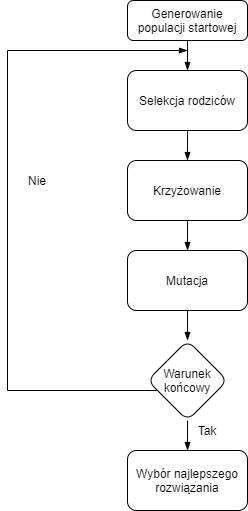
\includegraphics[scale=0.75]{grafika/algorytm_genetyczny.png}
	\caption{Schemat algorytmu genetycznego}
	\label{genetic}
\end{figure}
	
	Schemat blokowy klasycznego algorytm genetycznego zosta� pokazany na rysunku \ref{genetic}
	
	Pierwszym krokiem  jest wylosowanie populacji pocz�tkowej algorytmu. Wielko�� populacji podczas trwania ca�ego algorytmu jest sta�a $N$. Wa�ne jest, aby wszystkie osobniki by�y jak najbardziej zr�nicowane i wygenerowane losowo. Ka�dy z nich nast�pnie musi zosta� zakodowany do postaci chromosom�w, kt�re b�d� przechowywa� w sobie informacj� o odwiedzanych punktach w postaci gen�w.
	
	W populacji ka�dy osobnik musi zosta� poddany ocenie funkcji przystosowania. Jej wynik determinuje jak dobre jest dane rozwi�zanie. W klasycznym algorytmie d��y si� do maksymalizacji tej funkcji. Okre�lenie jak dana funkcja przystosowania b�dzie wygl�da�, jest to jedn� z najwa�niejszych cz�ci algorytmu genetycznego. Je�li zostanie �le zdefiniowana, znalezione osobnik mo�e nie spe�nia� wymaga� rozwi�zania problemu.
	
	Po ocenie osobnik�w zostaje sprawdzony warunek ko�cowy algorytmu. W zale�no�ci od problemu zostaje zdefiniowany inny warunek. W klasycznych podej�ciach s� dwa rodzaje warunk�w ko�cowych. Pierwszym popularnym warunkiem ko�cowym jest sta�a ilo�� iteracji algorytmu, czyli po wykonaniu okre�lonej ilo�ci razy ewolucji, wybierany jest najlepszy osobnik z populacji. Drugim warunkiem zazwyczaj jest przetwarzanie algorytmu dop�ki nie zostanie znaleziony dostatecznie dobry osobnik. Nale�y r�wnie� za�o�y�, �e je�li w kolejnych pokoleniach nie zachodzi poprawa najlepszego rozwi�zania, nale�y przerwa�. Wyb�r  w jaki spos�b b�dzie wygl�da� warunek ko�cowy zale�y od wielu czynnik�w. Je�li wa�ny jest kr�tki czas, nale�y za�o�y� pierwszy wariant. Je�li natomiast algorytm mo�e szuka� rozwi�zania nawet kilka godzin, mo�na przyj�� drugi wariant.
	
	Kolejnym krokiem algorytmu jest wyselekcjonowanie rodzic�w do reprodukcji. Polega ona na tym, �e osobniki lepsze(maj� wi�ksz� warto�� oceny przystosowania)maj� wi�ksze szans� na pozostanie rodzicem i przekazanie swoich cech. \cite{genetic_3}. Najpopularniejszymi metodami wyboru rodzic�w jest metoda ruletki oraz turniejowa.

\begin{figure}[h]
	\centering
	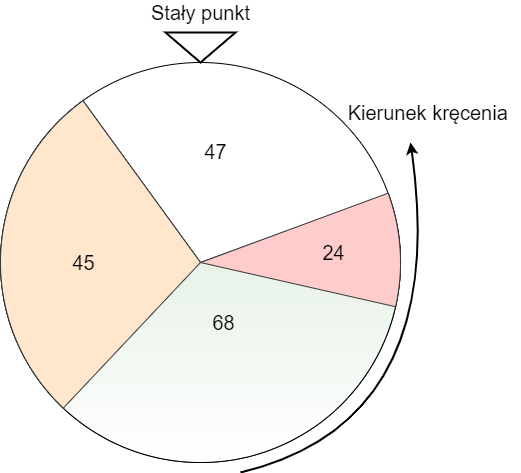
\includegraphics[scale=0.75]{grafika/ag_kolowy.png}
	\caption{Metoda ruletki}
	\label{ruletka}
\end{figure}
	Na rysunku \ref{ruletka} zosta�a zilustrowana pierwsza metoda ruletki. Ka�dy z osobnik�w dostaje wirtualny wycinek ko�a fortuny. Jego wielko�� zale�y od warto�ci funkcji prawdopodobie�stwa. Przy ka�dym wyborze rodzica nast�puje zakr�ceniem ko�a i do reprodukcji zostaje wybrany osobnik na kt�ry b�dzie wskazywa� sta�y punkt. 
	
	W metodzie turniejowej zostaje wybranych $r$ osobnik�w z populacji $N$. Z po�r�d nich zostaje wybrany zwyci�zca(najwi�ksza warto�� funkcji przystosowania), kt�ry trafia do puli rodzicielskiej.Im wi�ksza jest ilo�� osobnik�w $r$ tym mniejsze szanse, �e s�absze osobniki zostan� wybrane.
	
	Wybrani rodzice zostaj� poddani operatorom genetycznym: krzy�owanie(ang. crossover) oraz mutacji(ang. mutation). Krzy�owanie polega na po��czeniu cz�ci chromosomu jednego rodzica z cz�ci� drugiego. Wynikiem takiego po��czenia jest nowy osobnik. Proces krzy�owania w zale�no�ci mo�e przebiega� w r�ny ale zawsze okre�lony spos�b. Wszystko zale�y od metody zakodowania chromosomu oraz od tego czy kolejno�� gen�w i ich unikalno�� ma znaczenie. W klasycznym podej�ciu polega na rozci�ciu w dowolnym miejscu genotypu u dw�ch osobnik�w oraz skrzy�owaniu ich ze sob� w tym punkcie rys. \ref{crossover}.
\begin{figure}[h]
	\centering
	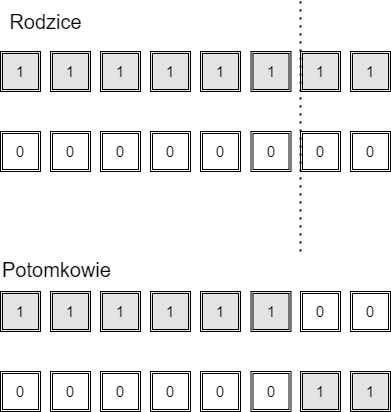
\includegraphics[scale=0.75]{grafika/ag_krzyzowanie.png}
	\caption{Klasyczne krzy�owanie}
	\label{crossover}
\end{figure}	
	 Nast�pnie u nowego osobnika mo�e z prawdopodobie�stwem $pm$ wyst�pi� mutacja. Jest to zmiana dowolnego pojedynczego rys \ref{mutacja} lub ci�gu gen�w na inny. Warto�� $pm$ w klasycznych algorytmach jest stosunkowo niskie. Mutacja ma na celu delikatne zr�nicowanie osobnik�w w celu przeszukania nowej przestrzeni rozwi�za�. Natomiast gdyby zachodzi�a cz�sto, mog�aby powodowa� niszczenie dobrych rozwi�za�.
	 \begin{figure}[h]
	\centering
	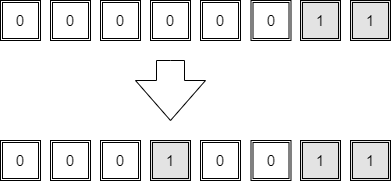
\includegraphics[scale=0.75]{grafika/ag_mutacja.png}
	\caption{Mutacja genotypu}
	\label{mutacja}
\end{figure}	
	
	Nast�pnie nowa populacja jest poddawana ocenie przystosowania i je�li wyst�pi� warunek ko�cowy, wybierane jest najlepsze rozwi�zanie. 


\section{Algorytm mrowkowy}

Obserwacje nad zachowaniami w przyrodzie wielokrotnie mia�y wp�yw na rozw�j nowych rozwi�za�. Tak jak w przypadku algorytmu genetycznego, tak i w przypadku algorytmu mr�wkowego pomys� zosta� zaczerpni�ty z przyrody. Dok�adne dzia�anie algorytmu mr�wkowego wzoruje si� na zachowaniu kolonii mr�wek. Dzi�ki pracy zespo�owej, owady te s� w stanie wypracowa� optymaln� �cie�k� mi�dzy siedliskiem a znalezionym pokarmem.

Dla niejednego gatunku problematyczne mog�oby by� odtworzenie przebytej �cie�ki. Na pocz�tku nale�a�oby zada� sobie pytanie w jaki spos�b te niewielkich rozmiar�w owady s� w stanie znacz�co u�atwi� sobie przetrwanie? Istotn� rol� odgrywa tutaj wspomniana ju� praca zespo�owa. To dzi�ki wsp�pracy mr�wki s� w stanie optymalizowa� tras�. Innym wa�nym czynnikiem determinuj�cym popraw� �cie�ki jest zapach jaki zostawiaj� mr�wki. 

Zapach nie jest niczym innym jak feromonem wytwarzanym przez mr�wki. Dzi�ki pozostawionemu zapachowi mr�wki wiedzia�y w jaki spos�b poruszali si� ich poprzednicy w zwi�zku z czym odtworzenie trasy nie stanowi�o ju� powa�nego problemu. Przy kolejnych iteracjach kolonia pr�buje optymalizowa� aktualn� tras�. W tym celu r�wnie� wykorzystuje zapach pozostawiony w poprzednich przej�ciach. �cie�ka jest losowo zmieniana w celu optymalizacji. Je�li modyfikacja przynios�a oczekiwany efekt, to trasa zostaje zmieniona. 

Feromony s� istotnym czynnikiem w ca�ym procesie. To dzi�ki nim trasa jest ulepszana. Zapach posiada jedn� z charakterystyk kt�ra na pocz�tku mo�e wydawa� si� problematyczna. Wraz z up�ywem czasu si�a zapachu s�abnie a� do ca�kowitego zanikni�cia. W�a�ciwo�� ta jest zalet�, a nie wad�. To dzi�ki pracy zespo�owej zapach na najlepszej trasie jest podtrzymywany, a na s�abszych zanika. Dzi�ki tej selekcji d�u�sze trasy nie s� brane pod uwag� w wyniku czego zostaje trasa najkorzystniejsza.

\subsection{Opis dzia�ania algorytmu}

Do wyznaczenia optymalnej trasy potrzebne s� d�ugo�ci jakie nale�y przeby� do przemieszczania si� mi�dzy punktami. W \ref{tabela_kosztow_ant} przedstawione s� przyk�adowe odleg�o�ci.

\begin{table}[htb]
\centering
\caption[Kr�tki podpis tabeli 1 -- do spisu tre�ci]{Warto�ci koszt�w}
\begin{tabular}{|c|c|c|c|c|}
\hline
  & A & B & C & D \\\hline
A & 0 & 3 & 8 & 2 \\\hline
B & 3 & 0 & 2 & 4 \\\hline
C & 8 & 2 & 0 & 1 \\\hline
D & 2 & 4 & 1 & 0 \\\hline
\end{tabular}
\label{tabela_kosztow_ant}
\end{table}

\begin{figure}[h]
	\centering
	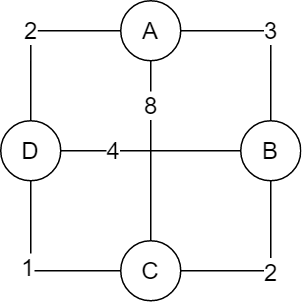
\includegraphics[scale=0.75]{grafika/kl_init_trasa_alg.png}
	\caption{Graf z wagami}
	\label{fig:kl_init_trasa_alg}
\end{figure}

R�wnie wa�ne jest wyznaczenie pocz�tkowych wsp�czynnik�w feromon�w. Na pocz�tku nadajmy wszystkim kraw�dziom w grafie warto�ci r�wne 1, a wsp�czynnik parowania niech wynosi 0.5.

\begin{table}[htb]
\centering
\caption[Kr�tki podpis tabeli 1 -- do spisu tre�ci]{Warto�ci feromon�w}
\begin{tabular}{|c|c|c|c|c|}
\hline
  & A & B & C & D \\\hline
A & 0 & 1 & 1 & 1 \\\hline
B & 1 & 0 & 1 & 1 \\\hline
C & 1 & 1 & 0 & 1 \\\hline
D & 1 & 1 & 1 & 0 \\\hline
\end{tabular}
\label{tabela_feromonow_ant}
\end{table}

\begin{figure}[h]
	\centering
	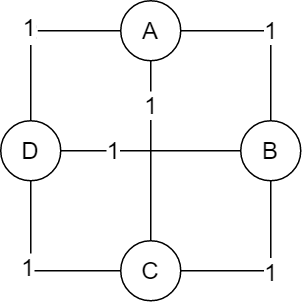
\includegraphics[scale=0.75]{grafika/kl_init_p_alg.png}
	\caption{Graf z pocz�tkowymi warto�ciami feromon�w}
	\label{fig:kl_init_trasa_alg}
\end{figure}

Posiadaj�c pocz�tkowe dane wyznaczmy w spos�b losowy trasy dla dw�ch agent�w: L1 i L2. Agent L1 porusza� si� tras� w kt�rej odwiedzi� wierzcho�ki w nast�puj�cej kolejno�ci: A, B, C, D, A. 

\begin{figure}[h]
	\centering
	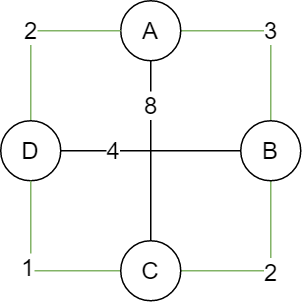
\includegraphics[scale=0.75]{grafika/kl_l1_trasa_alg.png}
	\caption{Trasa przebyta przez agenta L1}
	\label{fig:kl_init_trasa_alg}
\end{figure}

Agent L2 wyznaczy� nast�puj�c� tras�: A, C, B, D, A. 

\begin{figure}[h]
	\centering
	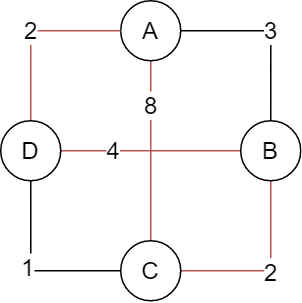
\includegraphics[scale=0.75]{grafika/kl_l2_trasa_alg.png}
	\caption{Trasa przebyta przez agenta L2}
	\label{fig:kl_init_trasa_alg}
\end{figure}

Mr�wki odpowiednio pokona�y dystans 8 i 16 punkt�w. Dzi�ki tej informacji mo�na zaktualizowa� warto�ci feromon�w na poszczeg�lnych kraw�dziach. Do oblicze� wykorzystany jest wz�r: TUTAJ WZ�R DODA�. Kraw�dzie A-B i C-D zosta�y odwiedzona jedynie przez agenta L1 w wyniku czego warto�� feromonu zostaje zmieniona na 10/16. Nast�pnie kraw�dzie A-C i B-D zostaj� zaktualizowane na 9/16. Kraw�dzie A-D i B-C s� odwiedzone dwukrotnie a warto�� feromon�w wynosi 11/16.

\begin{figure}[h]
	\centering
	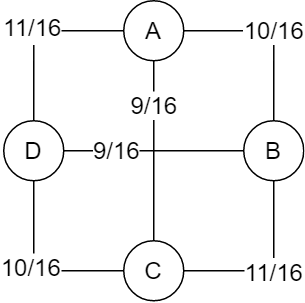
\includegraphics[scale=0.75]{grafika/kl_p_alg.png}
	\caption{Graf z warto�ciami feromon�w po modyfikacji}
	\label{fig:kl_init_trasa_alg}
\end{figure}

Ostatni� faz� algorytmu jest wyznaczenie prawdopodobie�stwa z jakim kolejni agenci b�d� wybiera� kolejny wierzcho�ek. W kolejnej iteracji agent L3 znajduje si� w wierzcho�ku B. Do wyboru ma kraw�dzie A, C i D. Wed�ug wzoru TUTAJ WZ�R DODA� wyliczane jest prawdopodobie�stwo dla wszystkich mo�liwo�ci. Przej�cie z kraw�dzi B do kraw�dzi A wynosi oko�o 20 PROCENT, do kraw�dzi D 30 procent, a do kraw�dzi C oko�o 50 PROCENT. 

Optymalna trasa zostanie wykszta�cona po wykonaniu wielu iteracji. Ilo�� iteracji nie jest zdefiniowana i dla ka�dego przypadku mo�e by� r�na. Sytuacja wygl�da identycznie w przypadku wyboru warto�ci p. Wa�ne jest natomiast to, aby w trakcie dzia�ania algorytmu nie modyfikowa� tej warto�ci. Powinno ona by� taka sama na ka�dym kroku algorytmu.

\section{Algorytm zachlanne}

\subsection{Metoda A*}
	
	
\subsection{Metoda A+}
	
\subsection{Metoda A-}
	


\chapter{Algorytm genetyczny - Pawe�}
	
\section{Chromosom}
	W algorytmie genetycznym, ka�dy osobnik z populacji reprezentuje jedno rozwi�zanie. Jako�� takiego rozwi�zania jest zapisywana do zakodowanej postaci chromosomu. Chromosom z definicji jest to ci�g gen�w reprezentuj�cy dane rozwi�zanie. Z kolei gen przenosi informacj� o cechach. Mo�liwo�� osi�gni�cia sukcesu w algorytmie genetycznym jest tylko wtedy, gdy odpowiednio zakoduje si� cechy i ustali funkcj� przystosowania. Do zakodowania badanego problemu zostanie u�yta metody permutacyjna, gdzie ka�dy punkt musi zosta� odwiedzony tylko raz. Ka�demu punktowi przed wylosowanie tras zostanie przypisany unikalny indeks, b�dzie on odpowiada� genowi. Nast�pnie dla ka�dego z $N$ osobnik�w zostanie zapisany chromosom w postaci ci�gu permutacyjnego. Na rysunku \ref{kodowanie} zosta�y zilustrowane przyk�ady kodowania permutacyjnego. Ka�dy chromosom musi zawiera� wszystkie geny.
	
\begin{figure}[h]
	\centering
	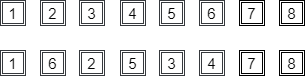
\includegraphics[scale=0.75]{grafika/chromosom.png}
	\caption{Kodowanie chromosom�w}
	\label{kodowanie}
\end{figure}
	
\section{Funkcja przystosowania}
	Algorytm genetyczny z definicji szuka osobnika z najwi�ksz� warto�ci� funkcji przystosowania. W badanym problemie nale�y znale�� najkr�tsz� tras�. W momencie, gdy d�ugo�� takiej trasy zostanie odwr�cona, to oka�e si�, �e im wi�ksza warto�� odwrotno�ci tym kr�tsza trasa. Zatem wz�r funkcji przystosowania to \[ fp = \frac{1}{s+1}\]	gdzie s - d�ugo�� trasy, czyli suma odleg�o�ci pomi�dzy genami(wierzcho�kami) 1 - 2 - 3 - 4 - 5 - 6 - 7.

\section{Metody krzy�owania}
	W pracy zostan� zbadane trzy rodzaje metod krzy�owania. Ka�de z nich charakteryzuje si� czym� innym je�li chodzi o liczb� potomk�w oraz porz�dek gen�w wzgl�dem rodzic�w. Geny mog� by� na takich samych pozycjach jak u przodk�w lub w ca�kowicie pomieszane.
\subsection{Krzy�owanie z cz�ciowym odwzorowaniem - PMX}
	PMX(ang. partially mapped crossover) jest odmian� krzy�owania dwupunktowego w kt�rym powstaje dw�jka potomstwa. Za��my, �e mamy wyselekcjonowanych dw�ch rodzic�w: 1 - 2 - 3 - 4 - 5 - 6 - 7 - 8 oraz 4 - 3 - 6 - 1 - 8 - 7 - 2 - 5 rys. \ref{krzyzowanie1}. 
\begin{figure}[h]
	\centering
	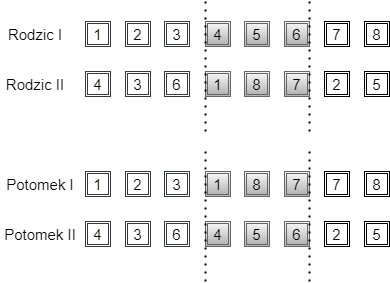
\includegraphics[scale=0.75]{grafika/krzyzowanie1.png}
	\caption{Krzy�owanie PMX cz�� 1}
	\label{krzyzowanie1}
\end{figure}

Losowane s� dwa dowolne punkty w kt�rych si� ich rozcina, w tym wypadku jest znajduj� si� one po trzecim i sz�stym genie. Powsta�e w ten spos�b segmenty pomi�dzy tymi punktami, s� to: 4 - 5 - 6 oraz 1 - 8 - 7, wymienia si� ze sob�. W wyniku tej operacji powsta�y dwa chromosomy: 1 - 2 - 3 - 1 - 8 - 7 - 7 - 8 oraz 4 - 3 - 6 - 4 - 5 - 6 - 2 - 5. Oba z nich nie s� permutacyjne i wyst�puj� w nich powt�rzenia. Nale�y je zamieni� na te geny, kt�re zosta�y wyci�te. W tym celu nast�puje okre�lenie relacji pomi�dzy genami w wyci�tych segmentach, kt�re nast�pnie si� zamienia ze sob� w chromosomach(rys. \ref{krzyzowanie2}).

\begin{figure}[h]
	\centering
	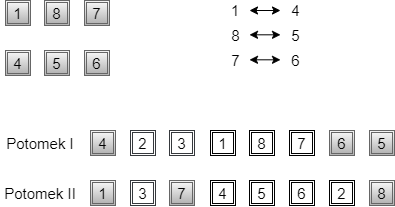
\includegraphics[scale=0.75]{grafika/krzyzowanie2.png}
	\caption{Krzy�owanie PMX cz�� 2}
	\label{krzyzowanie2}
\end{figure}

W pierwszym dziecku zamieniamy: 1 -> 4, 8 -> 5  oraz 7 -> 6. W drugim nale�y wykona� odwrotne mapowanie: 4 -> 1, 5 ->8 oraz 6 -> 7 Tak powsta�e dzieci posiadaj� ju� struktur� permutacyjn� i mog� bra� udzia� w kolejnych etapach.

\subsection{Krzy�owanie z zachowaniem porz�dku - OX}
	OX(ang. order crossover) jest r�wnie� odmian� krzy�owania dwupunktowego. W przeciwie�stwie do PMX wynikiem b�dzie tylko jedno dziecko. Rozwa�my rodzic�w z poprzedniego przyk�adu. Pierwszym krokiem jest wylosowanie dw�ch dowolnych punkt�w w kt�rych zostanie rozci�ty pierwszy rodzic. Za��my podobnie jak poprzednio, �e s� to punkty po trzecim i sz�stym genie(rys \ref{krzyzowanie3}). Oba punkty tworz� segment 4 - 5 - 6.
	
\begin{figure}[h]
	\centering
	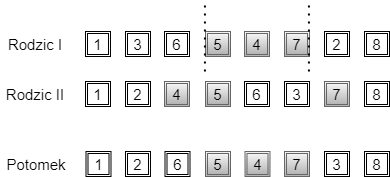
\includegraphics[scale=0.75]{grafika/krzyzowanie3.png}
	\caption{Krzy�owanie OX}
	\label{krzyzowanie3}
\end{figure}

	 Nast�pnie w drugim rodzicu nale�y usun�� geny, kt�re zosta�y z pierwszego rodzica wyci�te. Na rysunku \ref{krzyzowanie3} zosta�y one podkre�lone. Ostatnim krokiem jest wstawienie wycinka 4 - 5 - 6 do drugiego rodzica, w to samo miejsce z jakiego zosta�y usuni�te. Powsta� potomek 3 - 1 - 8 - 4 - 5 - 6 - 7 - 2. Na pierwszy rzut oka mo�na zauwa�y�, geny kt�re zosta�y wyci�te z pierwszego rodzica znajduj� si� na tych samych miejscach, pozosta�e natomiast si� przemie�ci�y.

\subsection{Krzy�owanie cykliczne - CX}
	CX(ang. cycle crossover) w przeciwie�stwie do PX i OX nie polega na krzy�owaniu w dw�ch okre�lonych punktach. Aby wyznaczy� potomka, nale�y w dowolnym rodzicu znale�� cykl permutacji, zaczynaj�c od dowolnego miejsca. Rozwa�my dwa chromosomy: 4 - 3 - 6 - 1 - 8 - 7 - 2 - 5 oraz 1 - 2 - 4 - 5 - 6 - 3 - 7 - 8(rys. \ref{krzyzowanie4}). Szukanie cyklu polega na kopiowaniu gen�w z jednego rodzica wed�ug pozycji okre�lonych przez rodzica drugiego. 
\begin{figure}[h]
	\centering
	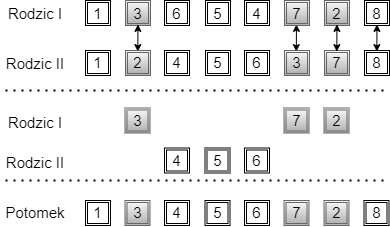
\includegraphics[scale=0.75]{grafika/krzyzowanie4.png}
	\caption{Krzy�owanie CX}
	\label{krzyzowanie4}
\end{figure}

	Za��my, �e zaczynamy od pierwszego genu czyli 4, jej odpowiednikiem w drugim rodzicu jest gen 1. Szukamy tego genu w pierwszym rodzicu. Znajduje si� on na czwartym miejscu, jej odpowiednikiem jest gen 5, kt�rego nast�pnie szukamy w pierwszym chromosomie. Czynno�� powtarzamy do momentu, a� zostanie wykryty cykl. W podanym przyk�adzie cykl wyst�puje dla 4 - 1 - 5 - 8- 6. Odpowiednikiem dla 6 genu jest ju� 4, wi�c zosta� wyznaczony cykl. Kolejnym krokiem jest wyci�cie cyklu z chromosomu, w kt�rym zosta� wyznaczony. W ten spos�b zostaje przepisane 4 - - 6 - 1 - 8 - - - 5.  Aby sko�czy� krzy�owanie, w puste miejsce nale�y wpisa� geny z drugiego rodzica, kt�re nie wyst�pi�y w cyklu. W tak powsta�ym dziecku 4 - 2 - 6 - 1 - 8 - 3 - 7 - 5, wszystkie geny zajmuj� tak� sam� pozycj� jak w kt�rym� z rodzic�w, inaczej ni� to by�o przy krzy�owaniu OX.


\section{Mutacje}
	W pracy zostan� zbadane trzy r�ne rodzaje mutacji. S� to specjalne mutacje wykorzystywane przy strukturach permutacyjnych. Ka�da z nich zostanie r�wnie� zbadana z r�n� warto�ci� pm. Z regu�y nie mo�e by� one du�e, aby nie niszczy� rozwi�za�. Powinno delikatnie wprowadza� r�norodno��, aby by�a mo�liwo�� odkry� w nowych obszarach. Bardzo wa�ne jest, aby zmiany nie zaburza�y struktury permutacyjnej chromosomu. Wszystkie mutacje zostan� opisane na tym samym chromosomie 1 - 2 - 3 - 4- 5 - 6 - 7 - 8.
	
\subsection{Mutacja odwracaj�ca}
	W mutacji odwracaj�cej wybierany jest dowolny podci�g gen�w z chromosomu, a nast�pnie ich kolejno�� jest odwracana. Za��my, �e wybrany podci�g to 3 - 4 - 5(rys. \ref{mutacja1}). W tym przypadku sk�ada si� on z trzech gen�w, wi�c po odwr�ceniu zamieni� si� dwa, �rodkowy zostanie na tym samym miejscu. Po mutacji ko�cowy chromosom ma posta� 1 - 2 - 5 - 4 - 3 - 6 - 7 - 8. Struktura permutacyjna nie zosta�a zachwiana. 
\begin{figure}[h]
	\centering
	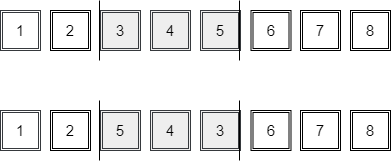
\includegraphics[scale=0.75]{grafika/mutacja1.png}
	\caption{Mutacja odwracaj�ca}
	\label{mutacja1}
\end{figure}
\subsection{Mutacja wstawiaj�ca}
	W tej mutacji dowolny gen jest przestawia si� w losowe miejsce. Jest to najprostsza mutacja, ale teoretycznie, mo�e tworzy� rozwi�zaniach w nowych przestrzeniach, gdy� je�li punkt, kt�ry znajduje si� na ko�cu trasy, mo�e znale�� si� na pocz�tku. Na rysunku \ref{mutacja2} zosta� wylosowany gen 5, kt�ry znajdowa� si� na pi�tym miejscu, po mutacji znalaz� si� na drugim miejscu, w rezultacie chromosom po mutacji to 1 - 5 - 2 - 3 - 4 - 6 - 7 - 8.
\begin{figure}[h]
	\centering
	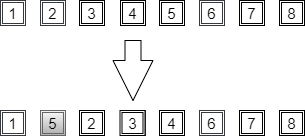
\includegraphics[scale=0.75]{grafika/mutacja2.png}
	\caption{Mutacja wstawiaj�ca}
	\label{mutacja2}
\end{figure}
\subsection{Mutacja zamieniaj�ca}
 	W mutacji zamieniaj�cej zamienia si� dwa dowolne geny miejscami. Jest to tak naprawd�, rozszerzona wersja mutacji wstawiaj�cej. Losujemy dwa dowolne geny, za��my, �e s� to 2 i 5, po czym zamieniamy je miejscami, tak jak na rysunku {\ref{mutacja3}}. Powsta�y chromosom to 1 - 5 - 3 - 4 - 2 - 6 - 7 - 8.
 \begin{figure}[h]
	\centering
	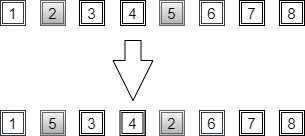
\includegraphics[scale=0.75]{grafika/mutacja3.png}
	\caption{Mutacja wstawiaj�ca}
	\label{mutacja3}
\end{figure}

	
\chapter{Algorytm mr�wkowy - Kamil}

S�owo rozw�j mo�e by� zestawiane z wieloma rzeczownikami. Wiele dziedzin ci�gle si� rozwija, powstaj� nowe udogodnienia kt�re wp�ywaj� na wiele dziedzin �ycia. Dzi�ki rozwojowi techniki ludzie s� w stanie osi�ga� cele, kt�re jeszcze nie dawno mog�y by� tylko marzeniami. 

Wykorzystuj�c prac� zespo�ow� mo�na w dok�adniejszy oraz szybszy spos�b udoskonala� rozwi�zanie. Wysi�ek wk�adany przez ka�d� jednostk� jest bardzo istotny. Mo�na naprawia� w�asne b��dy oraz korygowa� innych uczestnik�w zespo�u. Kontrola oraz wsp�praca na ka�dym etapie jest kluczem do sukcesu.

Obserwuj�c przyrod� mo�emy zauwa�y�, w jaki spos�b zwierz�ta radz� sobie z r�nymi problemami. Z�o�one grupy mog� by� spokojniejsze o zdobycie po�ywienia, czy te� o przetrwanie w ci�kich warunkach. Praca zespo�owa jest jedn� z cech, kt�rej osobniki w grupie ucz� si�, nie b�d�c nawet tego do ko�ca �wiadomym.

\section{Wprowadzenie do algorytmu}

Na przestrzeni czasu gatunki zwierz�t �yj�cych na ziemi przystosowa�o si� do panuj�cych tu warunk�w. Jedn� z takich gatunk�w s� mr�wki. Te niewielkich rozmiar�w owady posiadaj� zdolno�ci dzi�ki kt�rym s� w stanie dostosowywa� si� do otoczenia. Mr�wki �yj� w koloniach, w zwi�zku z czym wykorzystuj� prac� zespo�ow� do rozwi�zywania problem�w, jakie codziennie napotykaj� na swojej drodze.

Aby zapewni� przetrwanie kolonii, mr�wki potrzebuj� zapewni� sobie dost�p do pokarmu. Dziesi�tki tysi�cy mr�wek maj� swoje schronienie w mrowiskach. To tam trafia zdobyty przez nich pokarm. Wystarczy, aby jedna mr�wka znalaz�a miejsce z pokarmem, to po powrocie do mrowiska inne osobniki s� w stanie odtworzy� drog� do po�ywienia. Na tym etapie nale�a�oby si� zastanowi�, w jaki spos�b mr�wki s� w stanie komunikowa� si� mi�dzy sob�?

Jednym z opisywanych rozwi�za� do wyznaczania zoptymalizowanej trasy jest algorytm mr�wkowy, inaczej nazywany ACO - (ang. \textit{Ant Colony Optimization}). Jak sama nazwa wskazuje dzia�anie algorytmu jest zwi�zane z mr�wkami, a dok�adnie z koloni� mr�wek. Pomys� na algorytm zosta� zaproponowany na pocz�tku lat 90 XX wieku przez w�oskiego badacza - Marco Dorigo \cite{ant_intro}.

Mr�wki, dzi�ki pracy jak� wykonuj�, optymalizuj� przebyt� drog�. Chodzi dok�adnie o tras� jak� pokonuj� od swojego siedliska do miejsca, w kt�rym znajduje si� po�ywienie. Tras� kszta�tuje ca�a kolonia mr�wek, a nie pojedyncze przypadki. Mr�wki przebywaj�c ka�d� kolejn� podr� wykszta�caj� coraz to kr�tsz� tras�.

\section{Opis dzia�ania algorytmu}

Mr�wka w celu znalezienia pokarmu wyrusza z mrowiska bez obrania konkretnego kierunku. Losowo przesuwaj�c si� po terenie szuka pokarmu. Gdy ju� go znajdzie wraca do siedliska i informuje o tym fakcie pozosta�e mr�wki. Aby dostarczy� wi�cej pokarmu cz�� kolonii mr�wek wyrusza do miejsca spoczynku po�ywienia. Chc�c unikn�� sytuacji w kt�rej zdobycz mo�e zosta� zabrana przez inne owady, mr�wki musz� znale�� jak najkr�tsz� tras� jak� maj� do pokonania.

Mimo posiadania informacje o znalezionym pokarmie, ka�da mr�wka mo�e wyznaczy� na nowo lokalizacj� po�ywienia. Czy mr�wki poruszaj� si� t� sam� tras� przy ka�dym wyj�ciu z mrowiska? Aby trafi� do miejsca, w kt�rym znajduje si� pokarm, wspomniane owady wykorzystuj� �lady pozostawione przez osobnik�w, kt�re ju� natrafi�y na po�ywienie. W ten spos�b mr�wka, natrafia na �lad poprzednika, kt�ry jest wskaz�wk� do znalezienia poszukiwanego pokarmu. Wspomniany �lad nazywa si� feromonem. To dzi�ki tej w�a�ciwo�ci mr�wki s� w stanie lokalizowa� trasy prowadz�ce do pokarmu.

Na rysunku \ref{fig:kl_przyklad1} zosta� przedstawiony graf z wierzcho�kami A-B-C-D-E-F. Nad kraw�dziami kolorem czerwonym zosta�y oznaczone wagi. Na pocz�tku za��my, �e mamy do dyspozycji 80 agent�w. Przez \textit{K} pierwszych iteracji mr�wki porusza�y si� losowo i powsta� nast�puj�cy podzia�:

\begin{figure}[h!]
	\centering
	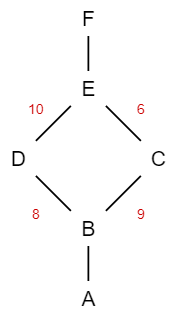
\includegraphics[scale=0.75]{grafika/kl_przyklad1}
	\caption{Po�o�enie �cie�ek na przyk�adowym grafie}
	\label{fig:kl_przyklad1}
\end{figure}

Tak jak mo�na to zauwa�y� na rysunku \ref{fig:kl_przyklad2}, po pierwszych iteracjach, przez obie �cie�ki przechodzi taka sama liczba agent�w. Dzieje si� tak, poniewa� mr�wki rozpoczynaj� prac� w spos�b losowy. W dalszych krokach nast�puj� modyfikacje i agenci d��� do wyznaczenia optymalnej �cie�ki.

\begin{figure}[h!]
	\centering
	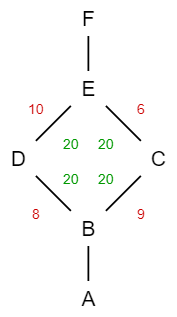
\includegraphics[scale=0.75]{grafika/kl_przyklad2}
	\caption{Rozk�ad agent�w na grafie po N pocz�tkowych iteracjach}
	\label{fig:kl_przyklad2}
\end{figure}

\begin{figure}[h!]
	\centering
	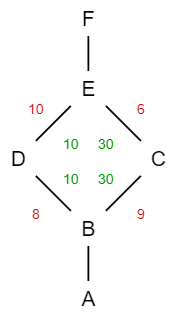
\includegraphics[scale=0.75]{grafika/kl_przyklad3}
	\caption{Rozk�ad agent�w w grafie po optymalizacji}
	\label{fig:kl_przyklad3}
\end{figure}

Liczba agent�w odwiedzaj�cych �cie�ki zmienia si�. Lepsza trasa zyskuje widoczn� przewag�. W kolejnych iteracjach mr�wki wykorzystuj� si�� feromon�w. Kr�tsze �cie�ki s� cz�ciej odwiedzane w zwi�zku z czym zapach na tych kraw�dziach jest silniejszy oraz podtrzymywany. Na d�u�szych trasach zapach zanika i przestaj� one by� atrakcyjne dla agent�w. Opisana sytuacja prowadzi do wyznaczenia trasy kt�ra jest najatrakcyjniejsza do przebycia dla mr�wek.

\section{Feromony}

Feromony posiadaj� cech�, kt�ra mo�e si� wydawa�, �e negatywnie wp�ywa na wyznaczanie �cie�ki. Chodzi tutaj o ulatnianie si� zostawionego zapachu. Na pocz�tku zjawisko to mo�e wydawa� si� niepo��danym, ale w rzeczywisto�ci ma du�y wp�ywa wyznaczenie kr�tszej trasy. Je�li feromony nie straci�yby na swojej sile, to bardzo prawdopodobne, �e pierwotna �cie�ka mog�aby zosta� uznana za bardziej atrakcyjn�.

W jaki spos�b wyznaczona zostaje najkr�tsza �cie�ka? Zapach feromon�w jest podtrzymywany przez w�druj�ce mr�wki. Z czasem owady te same zbaczaj� z drogi w celu poszukiwania alternatywnej trasy. Je�li wybrana trasa jest kr�tsza od pozosta�ych to �lad jest podtrzymywany, a na innych zanika. Dzi�ki temu w spos�b iteracyjny mo�na wyr�ni� tras� najkr�tsz�, a s�absze z czasem zostaj� odrzucone, poniewa� przestaj� by� odwiedzane.

Feromony s� istotnym czynnikiem w ca�ym procesie. To dzi�ki nim trasa jest ulepszana. Zapach posiada jedn� z charakterystyk, kt�ra na pocz�tku mo�e wydawa� si� problematyczna. Wraz z up�ywem czasu si�a zapachu s�abnie a� do ca�kowitego zanikni�cia. W�a�ciwo�� ta jest zalet�, a nie wad�. To dzi�ki pracy zespo�owej zapach na najlepszej trasie jest podtrzymywany, a na s�abszych zanika. Dzi�ki tej selekcji d�u�sze trasy nie s� brane pod uwag� w wyniku czego zostaje trasa najkorzystniejsza.

Do wyznaczenia optymalnej trasy potrzebne s� d�ugo�ci jakie nale�y przeby� do przemieszczania si� mi�dzy punktami. W tabeli \ref{tabela_kosztow_ant} przedstawione s� przyk�adowe odleg�o�ci.

\begin{table}[htb]
\centering
\caption[Warto�ci koszt�w]{Warto�ci koszt�w}
\begin{tabular}{|c|c|c|c|c|}
\hline
  & A & B & C & D \\\hline
A & 0 & 3 & 8 & 2 \\\hline
B & 3 & 0 & 2 & 4 \\\hline
C & 8 & 2 & 0 & 1 \\\hline
D & 2 & 4 & 1 & 0 \\\hline
\end{tabular}
\label{tabela_kosztow_ant}
\end{table}

R�wnie wa�ne jest wyznaczenie pocz�tkowych wsp�czynnik�w feromon�w. Na pocz�tku nadajmy wszystkim kraw�dziom w grafie warto�ci r�wne 1, a wsp�czynnik parowania niech wynosi 0.5. Jak zosta�y rozmieszczone warto�ci feromon�w na grafie mo�na zobaczy� na rysunku \ref{fig:kl_init_feromony}

\begin{figure}[h]
	\centering
	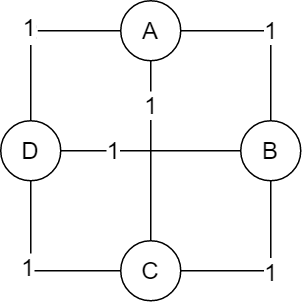
\includegraphics[scale=0.75]{grafika/kl_init_p_alg.png}
	\caption{Graf z pocz�tkowymi warto�ciami feromon�w}
	\label{fig:kl_init_feromony}
\end{figure}

Na rysunku \ref{fig:kl_init_trasa_alg} zosta� przedstawiony graf z warto�ciami feromon�w jakie s� pocz�tkowo umieszczone na kraw�dziach. Pocz�tkowe dane wyznaczmy w spos�b losowy trasy dla dw�ch agent�w: L1 i L2. Na rysunku \ref{fig:kl_trasa_l1} zosta�a przedstawiona trasa agenta L1. Odwiedzone zosta�y wierzcho�ki w nast�puj�cej kolejno�ci: A, B, C, D, A. 

\begin{figure}[h]
	\centering
	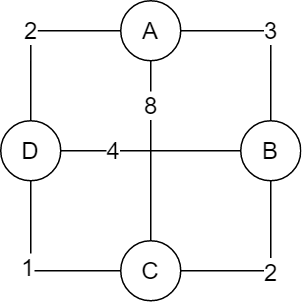
\includegraphics[scale=0.75]{grafika/kl_init_trasa_alg.png}
	\caption{Graf z wagami}
	\label{fig:kl_init_trasa_alg}
\end{figure}

\begin{figure}[h]
	\centering
	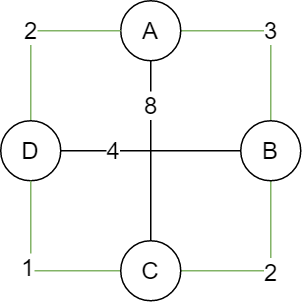
\includegraphics[scale=0.75]{grafika/kl_l1_trasa_alg.png}
	\caption{Trasa przebyta przez agenta L1}
	\label{fig:kl_trasa_l1}
\end{figure}

Agent L2 wyznaczy� nast�puj�c� tras�: A, C, B, D, A. Trasa ta zosta�a przestawiona na rysunku \ref{fig:kl_trasa_l2}.

\begin{figure}[h]
	\centering
	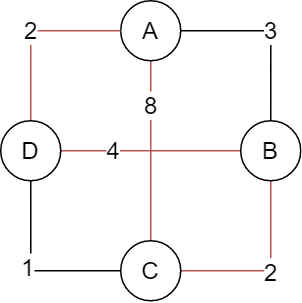
\includegraphics[scale=0.75]{grafika/kl_l2_trasa_alg.png}
	\caption{Trasa przebyta przez agenta L2}
	\label{fig:kl_trasa_l2}
\end{figure}

Mr�wki odpowiednio pokona�y dystans 8 i 16 punkt�w. Dzi�ki tej informacji mo�na zaktualizowa� warto�ci feromon�w na poszczeg�lnych kraw�dziach. Do oblicze� wykorzystany jest wz�r: \\
\begin{equation}
\tau\textsubscript{i,j}=((1-p)\tau\textsubscript{i,j}+\sum\limits_{k=1}^m \Delta\tau_{i,j}^k)
\end{equation}

gdzie: \\
-- \textit{p} jest wsp�czynnikiem parowania feromon�w;\\
-- \textit{i} jest wierzcho�kiem pocz�tkowym;\\
-- \textit{j} jest wierzcho�kiem docelowym;\\
-- \textit{k} jest wag� mi�dzy punktami;\\

Kraw�dzie A-B i C-D zosta�y odwiedzona jedynie przez agenta L1 w wyniku czego warto�� feromonu zostaje zmieniona na 10/16. Nast�pnie kraw�dzie A-C i B-D zostaj� zaktualizowane na 9/16. Kraw�dzie A-D i B-C s� odwiedzone dwukrotnie a warto�� feromon�w wynosi 11/16. Aktualne rozmieszczenie warto�ci feromon�w zosta�o przedstawione na rysunku \ref{fig:kl_feromony1}.

\begin{figure}[h]
	\centering
	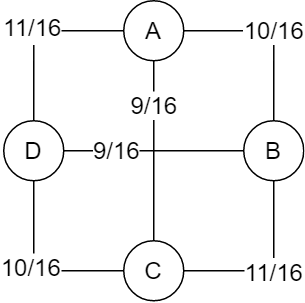
\includegraphics[scale=0.75]{grafika/kl_p_alg.png}
	\caption{Graf z warto�ciami feromon�w po modyfikacji}
	\label{fig:kl_feromony1}
\end{figure}

Ostatni� faz� algorytmu jest wyznaczenie prawdopodobie�stwa z jakim kolejni agenci b�d� wybiera� kolejny wierzcho�ek. W kolejnej iteracji agent L3 znajduje si� w wierzcho�ku B. Do wyboru ma kraw�dzie A, C i D. Dla wszystkich mo�liwo�ci wyliczane jest prawdopodobie�stwo wed�ug wzoru\\
\begin{equation}
p\textsubscript{i,j}=\frac{(\tau\textsubscript{i,j})(\eta\textsubscript{i,j})}{\sum(\tau\textsubscript{i,j})(\eta\textsubscript{i,j}))})
\end{equation}
gdzie:\\
-- \textit{i} jest wierzcho�kiem pocz�tkowym;\\
-- \textit{j} jest wierzcho�kiem docelowym;\\
 
Prawdopodobie�stwo przej�cia z kraw�dzi B do kraw�dzi A wynosi oko�o 20\%, do kraw�dzi D 30\%, a do kraw�dzi C oko�o 50\%. 

Optymalna trasa zostanie wyznaczona po wykonaniu wielu iteracji. Liczba iteracji nie jest zdefiniowana i dla ka�dego przypadku mo�e by� r�na. Sytuacja wygl�da identycznie w przypadku wyboru warto�ci p. Wa�ne jest natomiast to, aby w trakcie dzia�ania algorytmu nie modyfikowa� tej warto�ci. Powinno ona by� taka sama na ka�dym kroku algorytmu.


\chapter{Algorytmy zach�anne -- PN}
	Istnieje wiele algorytm�w zach�annych, pozwalaj�cych otrzyma� optymalne rozwi�zanie dla problemu znalezienia najkr�tszej trasy. W poni�szym rozdziale opisane dok�adniej zosta�o dzia�anie algorytmu najbli�szego s�siada, algorytmu najmniejszej kraw�dzi oraz algorytmu A*. W celu zoptymalizowania otrzymanych rozwi�za� zastosowany zostanie operator 2-opt oraz wsp�czynnik b��du przy dokonywaniu wybor�w.

\section{Algorytm najbli�szego s�siada}
	Poni�szy podrozdzia� przybli�y dzia�anie algorytmu najbli�szego s�siada. Wszystkie wymagane dla algorytmu operacje zostan� opisane krok po kroku oraz przedstawione na~ kr�tkim przyk�adzie. 
	
	Jak sama nazwa wskazuje algorytm najbli�szego s�siada jest to algorytm polegaj�cy na~ odwiedzaniu, zaczynaj�c od wybranego wierzcho�ka pocz�tkowego, nast�pnego wierzcho�ka jeszcze nieodwiedzonego znajduj�cego si� najbli�ej poprzednio odwiedzonego. 

\begin{figure}[h]
	\centering
	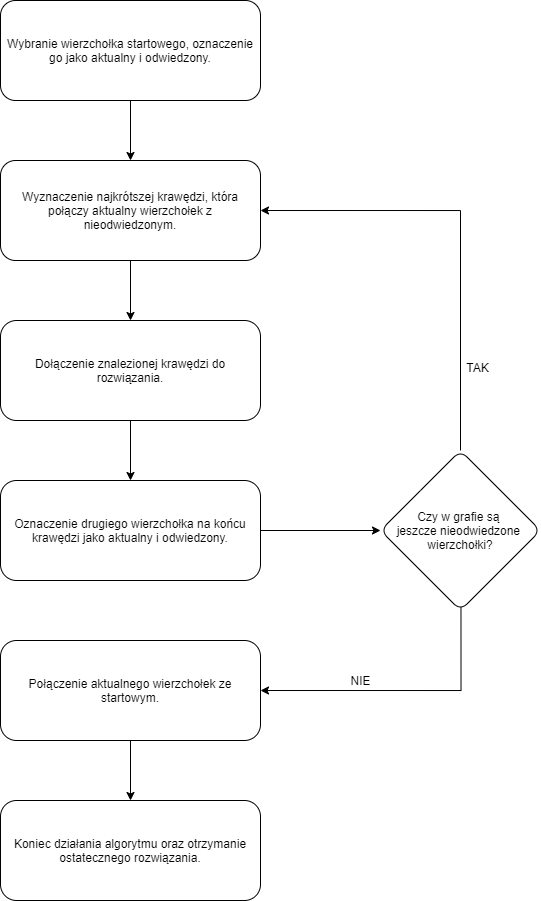
\includegraphics[scale=0.5]{grafika/ans_graph.png}
	\caption{Schemat algorytmu najbli�szego s�siada}
	\label{nearest_neighbour}
\end{figure}

Na rysunku \ref{nearest_neighbour} zosta� pokazany schemat blokowy algorytmu najbli�szego s�siada. Pierwszym krokiem jest wyznaczenie wyznaczenie wierzcho�ka startowego. Nast�pnie dla~ aktualnego wierzcho�ka nale�y obliczy� najkr�tsz� kraw�d� ��cz�c� aktualny wierzcho�ek spo�r�d kolekcji wierzcho�k�w nieodwiedzonych. Najlepsz� opcje po��czenia dw�ch wierzcho�k�w nale�y doda� do rozwi�zania, a od~ drugiego wierzcho�ka algorytm b�dzie wyznacza� kolejne odleg�o�ci od nieodwiedzonych jeszcze wierzcho�k�w. Czynno�ci nale�y powtarza� do momentu odwiedzenia wszystkich wierzcho�k�w w podanym grafie. Na samym ko�cu wystarczy jedynie po��czy� ostatni wierzcho�ek z pocz�tkowym. Po~ wykonaniu wszystkich krok�w, algorytm najbli�szego s�siada powinien zwr�ci� optymalne rozwi�zanie.

\begin{figure}[h]
	\centering
	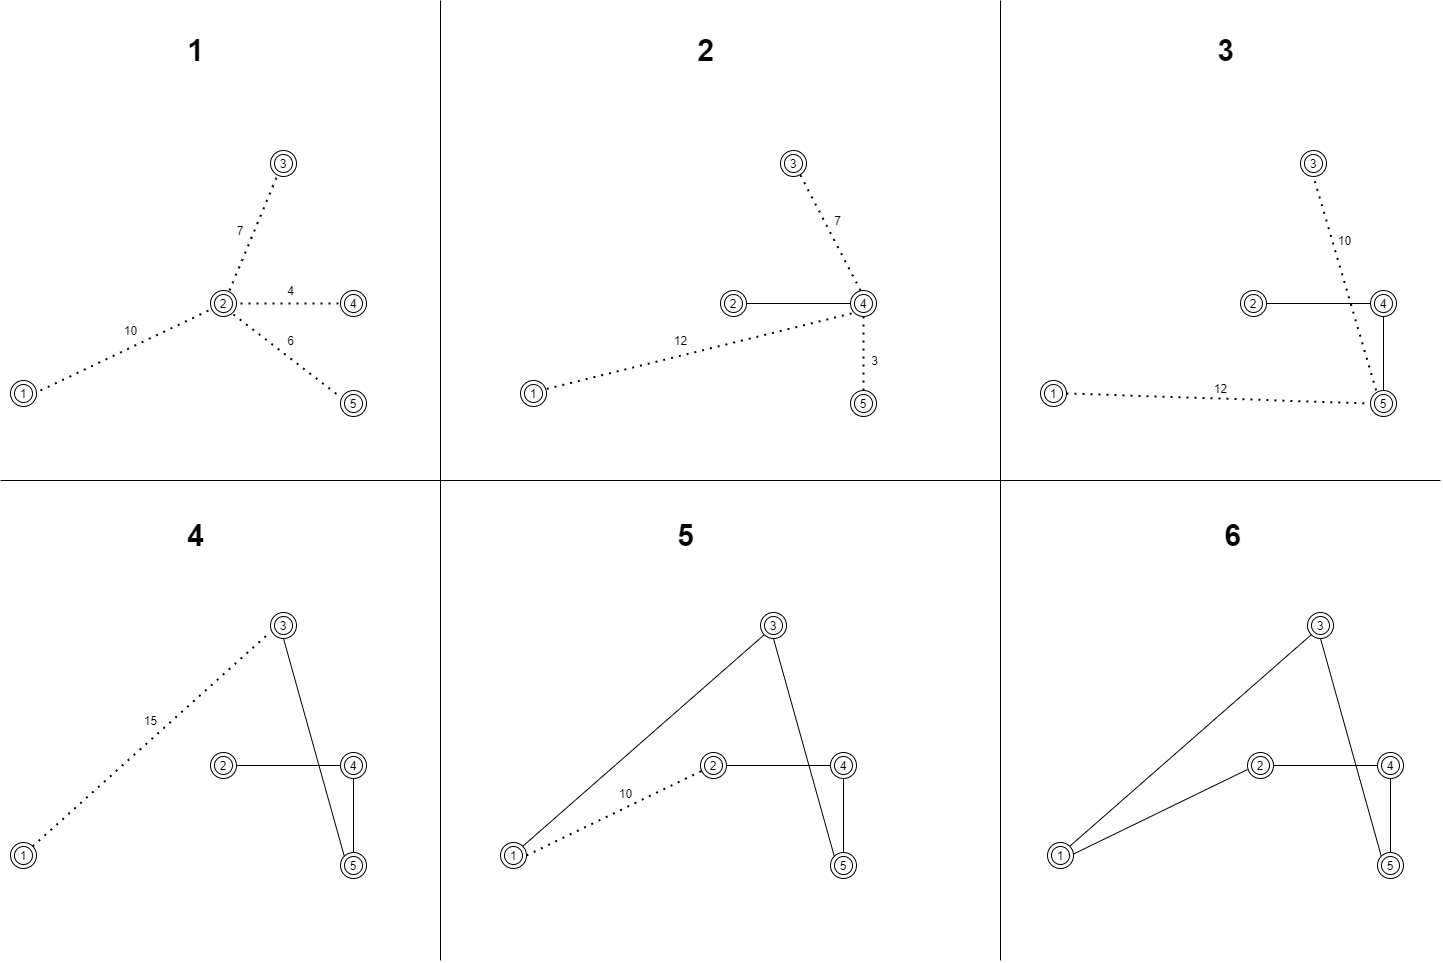
\includegraphics[scale=0.3]{grafika/ans_last.png}
	\caption{Algorytm najbli�szego s�siada}
	\label{nearest_neighbour_inaction}
\end{figure}

	Aby lepiej zobrazowa� rozwi�zanie otrzymane przez algorytm przedstawiono poni�ej na rysunku \ref{nearest_neighbour_inaction} jego dzia�anie na przyk�adzie. W podanym przypadku nale�y za�o�y�, �e wierzcho�ek numer 2 jest wierzcho�kiem startowym, wi�c nale�y ustawi� go jako aktualny w danym momencie. Po obliczeniu wszystkich odleg�o�ci prowadzonych do wierzcho�k�w nieodwiedzonych wychodzi, �e najkr�tsza kraw�d� prowadzi do wierzcho�ka numer 4, wi�c nale�y do��czy� wybrana kraw�d� do rozwi�zania i oznaczy� nowy aktualny wierzcho�ek, kt�ry staje si� r�wnie� odwiedzonym. 
	
	W podanym grafie znajduj� si� nadal nieodwiedzone wierzcho�ki, dlatego algorytm powtarza krok numer 2 w celu znalezienia kolejnej najkr�tszej kraw�dzi. Kolejn� najlepsz� odnalezion� w danym momencie kraw�dzi�, kt�r� algorytm doda do rozwi�zania b�dzie kraw�d� o warto�ci 3 ��cz�ca aktualny wierzcho�ek z wierzcho�kiem numerr 5. Kroki 4, 5 oraz 6 przedstawiaj� kolejne powtarzalne iteracje algorytmu dochodz�c w ostatnim kroku do~ utworzenia cyklu i tym zako�czeniu dzia�ania algorytmu. W ten spos�b otrzymano zach�anne rozwi�zanie 2 - 4 - 5 - 3 - 1 - 2. Warto zaznaczy�, �e dzi�ki oznaczaniu wierzcho�k�w jako odwiedzone nie trzeba w �adnej iteracji martwi� si� o to czy do��czenie kolejnej kraw�dzi z nieodwiedzonym wierzcho�kiem spowoduje utworzenie niepo��danego cyklu.

\section{Algorytm najmniejszej kraw�dzi}
	Kolejny podrozdzia� algorytm�w zach�annych zosta� po�wi�cony dok�adniejszemu opisowi dzia�ania algorytmu najmniejszej kraw�dzi, kt�ry w swoim dzia�aniu przypomina algorytm poszukuj�cy minimalnego drzewa rozpinaj�cego, poprzez do��czenie do aktualnego rozwi�zania najkr�tszych w�r�d dopuszczalnych kraw�dzi.	Aby otrzyma� zach�anne rozwi�zanie przy wykorzystaniu algorytmu najmniejszej kraw�dzi nale�y wykona� nast�puj�ce kroki przedstawione schemacie blokowym na rysunku \ref{ank}.
	
\begin{figure}[h]
	\centering
	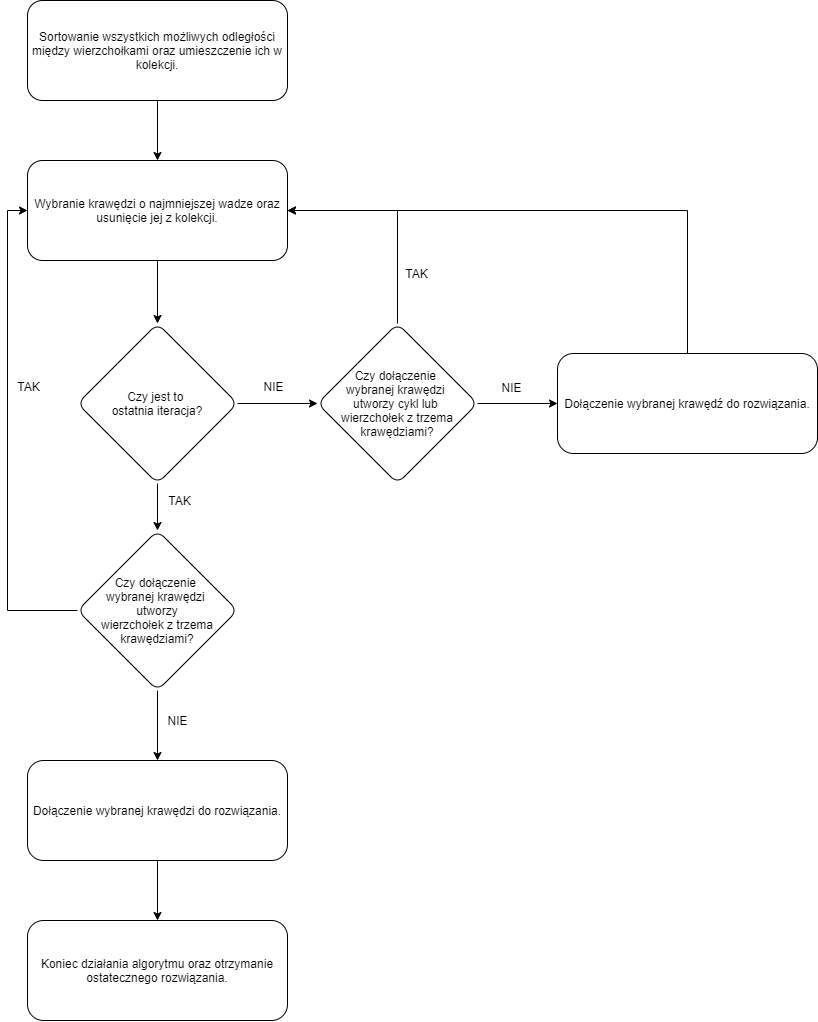
\includegraphics[scale=0.4]{grafika/ank_graph.png}
	\caption{Schemat algorytmu najmniejszej kraw�dzi}
	\label{ank}
\end{figure}

Algorytm rozpoczyna swoje dzia�anie od posortowania wag kraw�dzi mi�dzy wszystkimi wierzcho�kami oraz umieszcza podane odleg�o�ci w kolekcji. Nast�pnie wybierana jest zawsze kraw�d� o najmniejszej warto�ci oraz od razu usuwana jest ona z podanej kolekcji. Aby wybrane po��czenie mi�dzy wierzcho�kami zosta�o dodane do rozwi�zania musi, spe�nia� warunek nie utworzenia cyklu oraz wierzcho�ka o trzech kraw�dziach, w~ przeciwnym wypadku po��czenie jest pomijane oraz algorytm wybiera kolejn� kraw�d�. Iteracje s� powtarzane do momentu, a� liczba dodanych po��cze� jest r�wna liczbie wszystkich wierzcho�k�w. W przypadku ostatniej iteracji wyznaczona kraw�d� nie musi ju� spe�nia� warunku z utworzeniem cyklu. Po zako�czeniu dzia�ania algorytmu rozwi�zanie dla~ algorytmu najmniejszej kraw�dzi jest optymalne.
	
\begin{figure}[h]
	\centering
	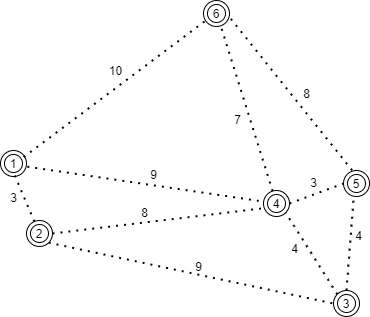
\includegraphics[scale=0.5]{grafika/ank_initial_finish.png}
	\caption{Pocz�tkowe rozmieszczenie wierzcho�k�w}
	\label{ank_initial}
\end{figure}

Dzia�anie algorytmu przedstawione zosta�o na rysunku \ref{ank_initial} przedstawiaj�cym przyk�ad ze sze�cioma losowo rozmieszczonymi wierzcho�kami. Natomiast wizualizacja kolejnych krok�w algorytmu zosta�a przedstawiona na rysunku \ref{ank_final}. Po posortowaniu wszystkich dost�pnych kraw�dzi dla ka�dego wierzcho�ka mo�na rozpocz�� dzia�anie algorytmu.
	
\begin{figure}[h]
	\centering
	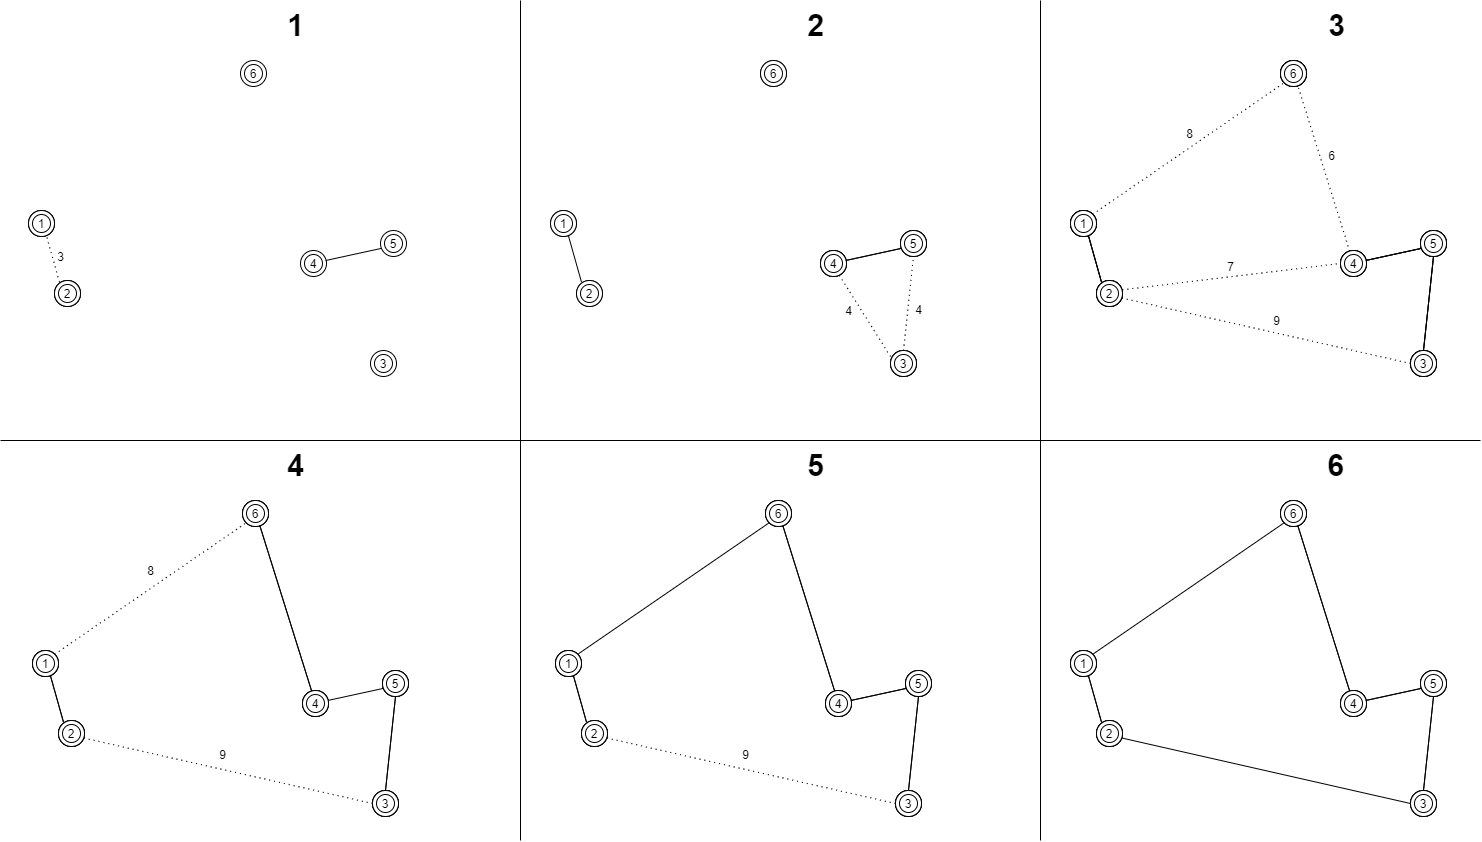
\includegraphics[scale=0.30]{grafika/ank_steps_final.png}
	\caption{Algorytm najmniejszej kraw�dzi}
	\label{ank_final}
\end{figure}

	Podczas pierwszej iteracji okazuje si�, �e s� aktualnie dwie kraw�dzie z najmniejsz� wag� o warto�ci 3 (1 - 2 oraz 4 - 5), nie ma wi�c znaczenia, kt�ra kraw�d� algorytm doda w pierwszej kolejno�ci, poniewa� �adna z wybranych nie utworzy w tym momencie cyklu. W przypadku drugiej iteracji algorytm wybiera kraw�d� o najmniejszej wadze, do��czaj�c j� do aktualnego rozwi�zania. Analogiczna sytuacja do pierwszej iteracji wyst�puje w trzeciej iteracji, gdzie nie ma r�nicy, kt�ra kraw�d� zostanie do��czona do rozwi�zania. Czwarta iteracja pokazuje sytuacj�, w kt�rej nie mo�na po��czy� kraw�dzi 3 - 4, poniewa� utworzy�oby to niedozwolony w trakcie algorytmu cykl, dlatego tym razem wybierane jest inne po��czenie o najmniejszej wadze (4 - 6). 
	
	Kolejny krok przedstawia przedstawia przypadek, gdzie nie jest mo�liwe po��czenie kraw�dzi 2 - 4 (najmniejsza warto�� - 7), poniewa� spowodowa�oby dla wierzcho�ka nr 4 utworzenie trzech wychodz�cych z niego kraw�dzi, wi�c do rozwi�zania dochodzi kolejna najmniejsza kraw�d� 1 - 6. 
	
	W ostatnim kroku, pomimo dost�pnych kraw�dzi z mniejsz� wag� wybierana zosta�a kraw�d� 2 - 3, poniewa� tylko ona nie spowoduje utworzenia wierzcho�ka o trzech kraw�dziach. W takim wypadku ko�cz�c dzia�anie algorytmu otrzymano rozwi�zanie 1 - 6 - 4 - 5 - 3 - 2 - 1.
	
\section{Algorytm A*}
	Ostatnim om�wionym rozwi�zaniem do znajdowania najkr�tszej �cie�ki w grafie jest algorytm A*, w kt�rym zawsze zostanie znalezione najkorzystniejsze zach�anne rozwi�zanie. Strategia gwarantuje, �e ka�dy wierzcho�ek zostanie odwiedzony, przy czym dokonuje w danym momencie najlepszych wybor�w. 
	
	G��wn� zasad� algorytmu A* jest minimalizacja funkcji kosztu $g(x)$ oraz funkcji heurystycznej $h(x)$ zdefiniowanej jako funkcja celu $f(x)=g(x)+h(x)$. Funkcja heurystyczna musi spe�nia� dwa wymagane warunki tj. warunek dopuszczalno�ci i warunek monotoniczno�ci. Warunek dopuszczalno�ci polega na tym, aby funkcja heurystyczna stara�a si� minimalizowa� koszt. Natomiast warunek monotoniczno�ci m�wi, �e oszacowywanie wyniku musi by� coraz mniej optymistyczne w momencie zbli�ania si� do rozwi�zania. Je�li przestrze� przeszukiwa� zawiera� b�dzie �cie�ki, mo�na w�wczas sprowadzi� problem do problemu poszukiwania najkr�tszej �cie�ki w grafie. W danym przypadku funkcj� heurystyczn� b�dzie odleg�o�� w linii prostej mi�dzy wierzcho�kami.
	
\begin{figure}[h]
	\centering
	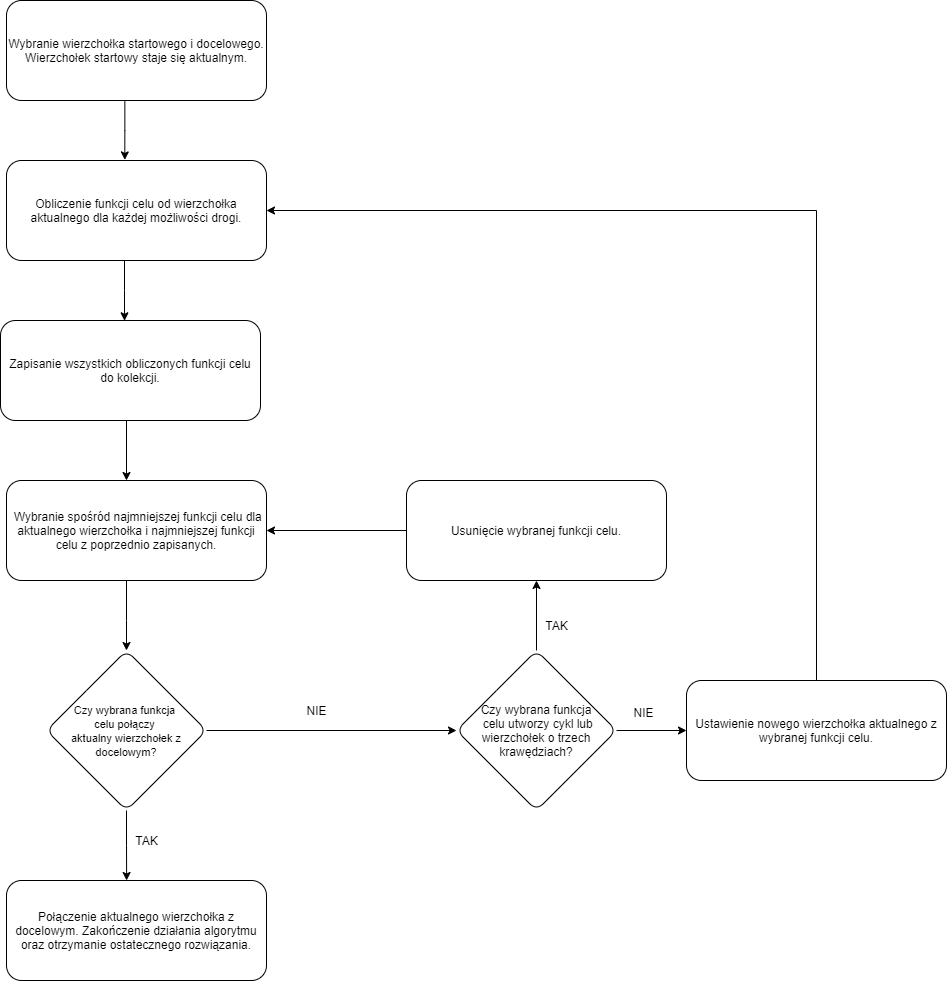
\includegraphics[scale=0.4]{grafika/astar_schema.png}
	\caption{Schemat blokowy algorytmu A*}
	\label{astar_schema}
\end{figure}	
	
Schemat blokowy dzia�ania algorytmu A* zosta� przedstawiony na rysunku \ref{astar_schema}. Algorytm rozpoczyna swoje dzia�anie od wyboru wierzcho�ka startowego oraz ko�cowego, gdzie wierzcho�ek startowy staje si� aktualnym. Nast�pnie dla aktualnego wierzcho�ka obliczana i zapisywana jest funkcja celu $f(x)$ dla ka�dego poszczeg�lnego mo�liwego po��czenia. Kolejnym krokiem jest wybranie spo�r�d minimalnej funkcji celu dla aktualnego wierzcho�ka oraz minimalnej funkcji celu z poprzednio zapisanych (je�li takowe istniej�). Je�li wybrana funkcja celu nie ��czy aktualnego wierzcho�ka z docelowym oraz nie utworzy cyklu lub wierzcho�ka o trzech kraw�dziach jest brana dalej pod uwag� i ustalany jest nowy aktualny wierzcho�ek. W przeciwnym wypadku, wybrana funkcja celu nie jest brana pod uwag� i algorytm jeszcze raz por�wnuje obliczone poprzednio warto�ci funkcji celu. Kroki algorytmu s� powtarzane do momentu a� wybrana funkcja celu po��czy aktualny wierzcho�ek z ko�cowym.


\begin{figure}[h]
	\centering
	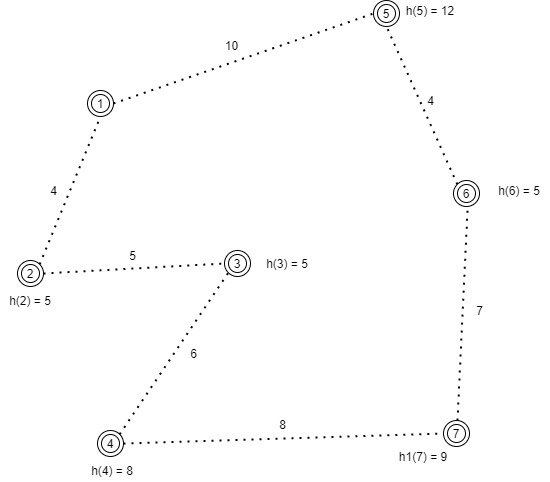
\includegraphics[scale=0.4]{grafika/astar_initial.png}
	\caption{Graf u�yty do przedstawienia dzia�ania algorytmu A*}
	\label{astar_initial}
\end{figure}

Wizualizacja dzia�ania algorytmu A* zosta�a przedstawiona na grafie umieszczonym na rysunku \ref{astar_initial}. Wierzcho�kiem startowym b�dzie w tym wypadku wierzcho�ek numer 1, natomiast wierzcho�kiem docelowym b�dzie punkt numer 7. Jak mo�na zauwa�y�, na rysunku \ref{astar_final} podczas pierwszej iteracji algorytm A* zdefiniowa� dwie funkcje celu, jednak�e $f1(2)=4+5$ jest w danym momencie lepszym wyborem. W kolejnej iteracji nadal rozwini�cie pierwszej funkcji celu daje lepszy rezultat, dlatego te� nowym aktualnym wierzcho�kiem staje si� wierzcho�ek numer 3. Trzecia iteracja przedstawia sytuacje, w kt�rej druga funkcja celu ��cz�ca aktualny wierzcho�ek z wierzcho�kiem numer 5 daje lepszy w danym momencie rezultat, dlatego wierzcho�ek numer 5 jest brany pod uwag�. Po zastosowaniu si� do za�o�e� algorytmu oraz wykonaniu wszystkich krok�w otrzymujemy optymalne rozwi�zanie ��cz�ce wierzcho�ek numer 1 z wierzcho�kiem numer 7(1 - 5 - 6 - 7) o warto�ci 21.


\begin{figure}[h]
	\centering
	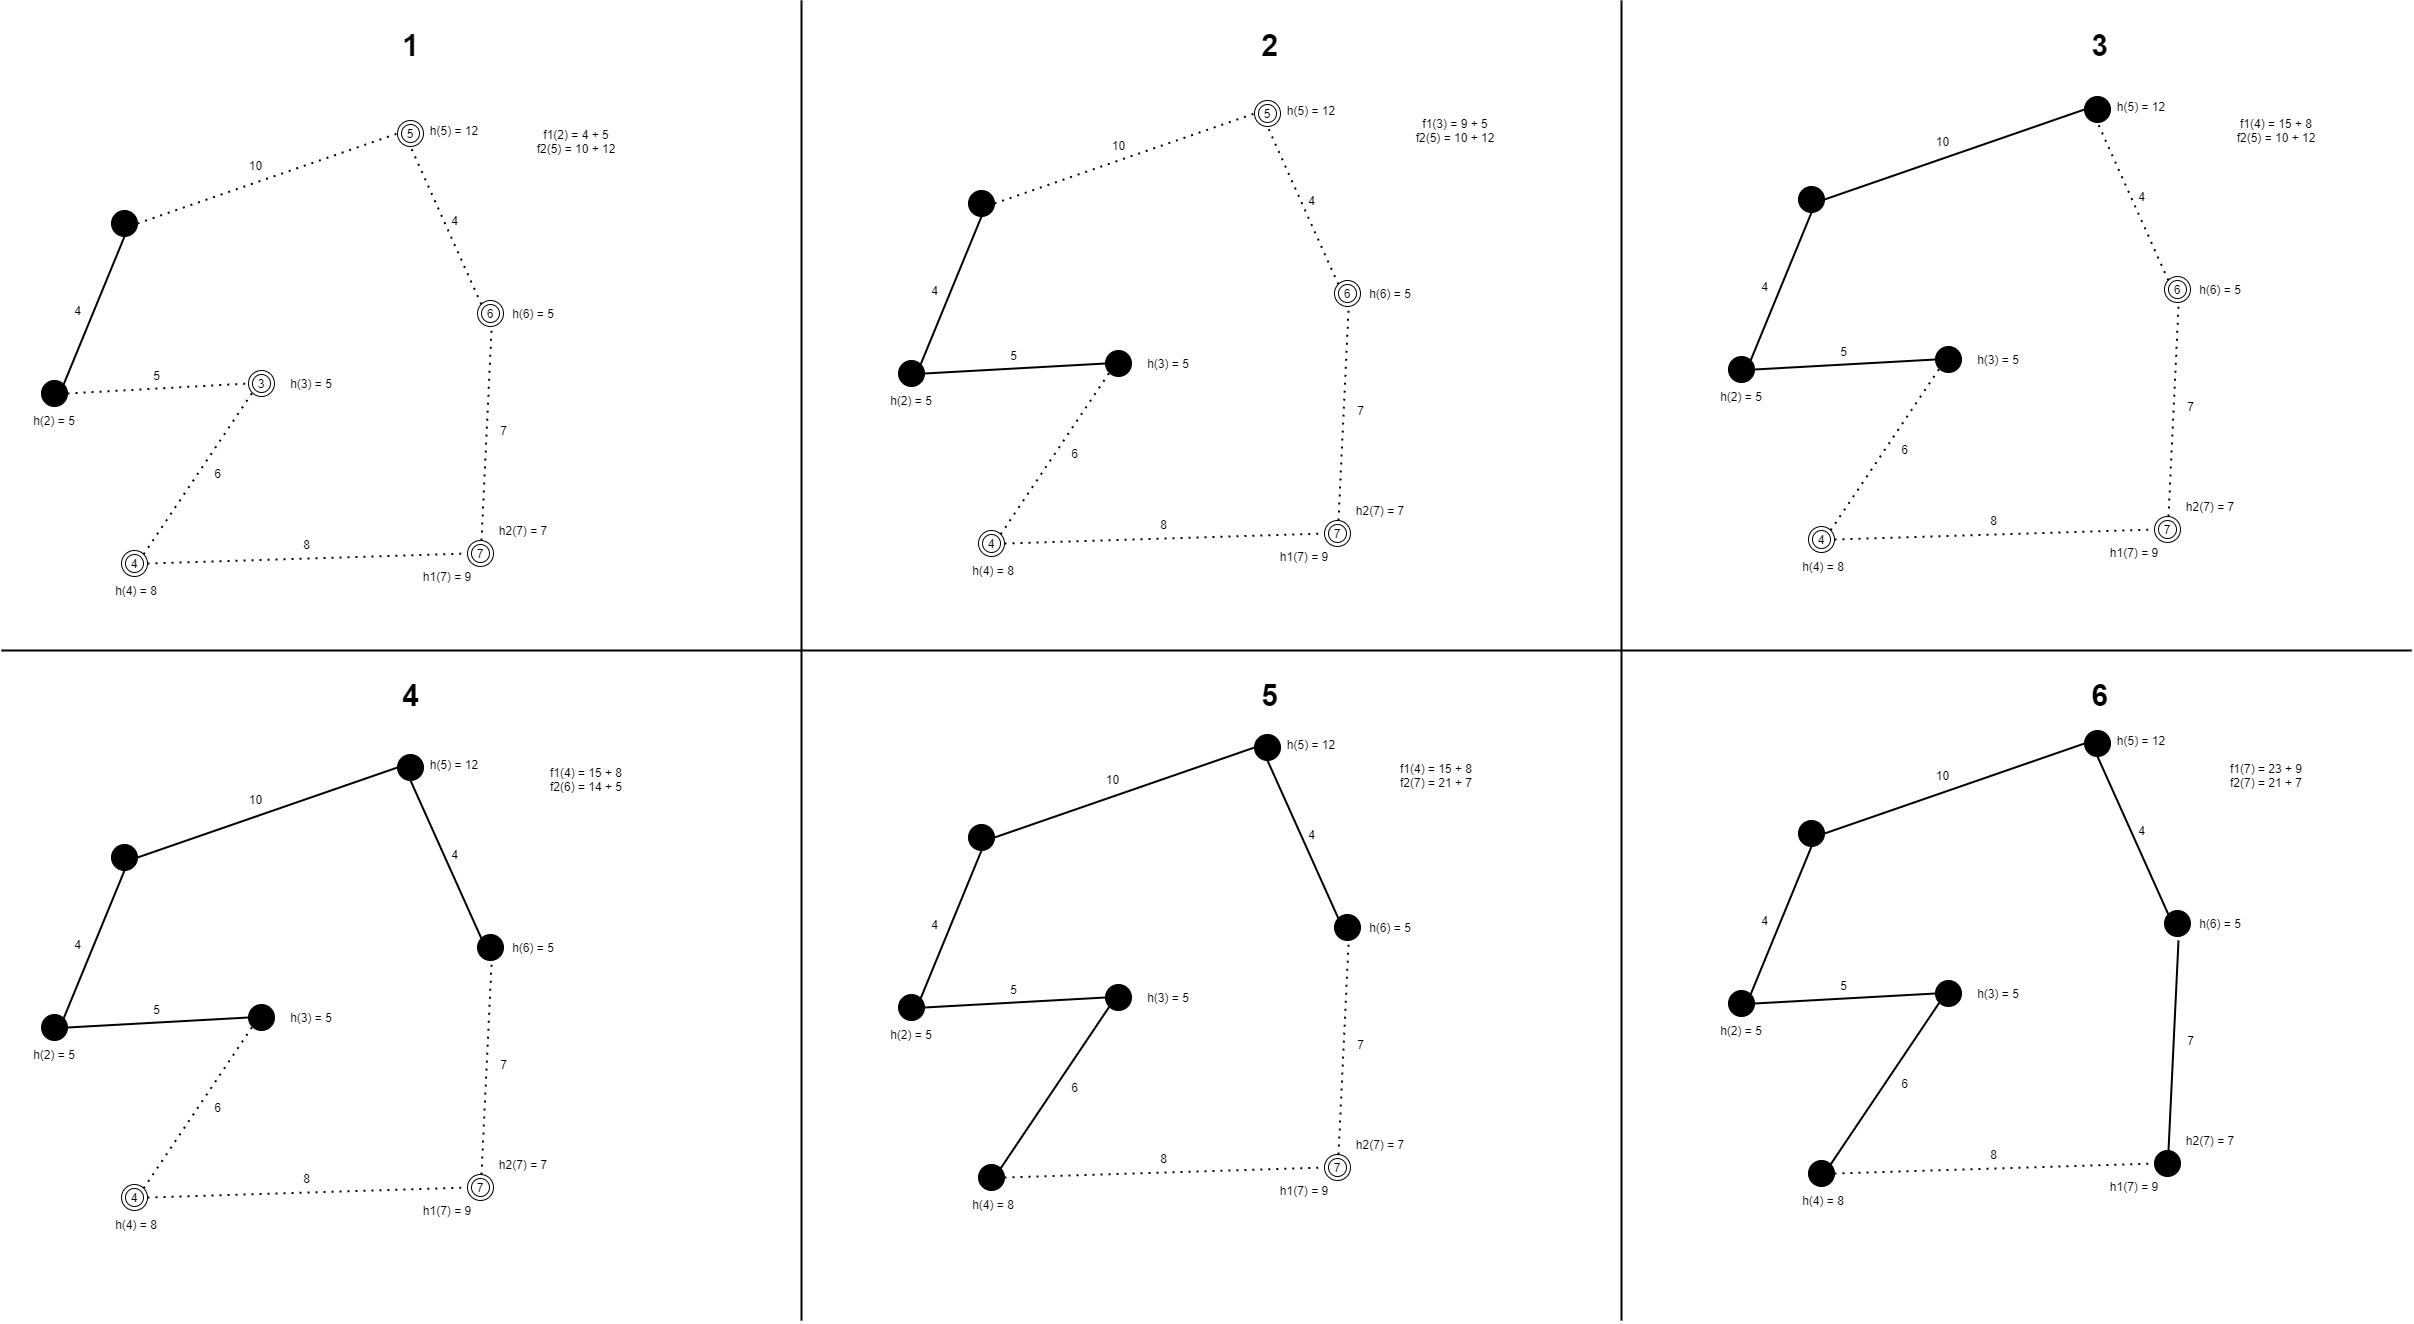
\includegraphics[scale=0.2]{grafika/astar_final.png}
	\caption{Poszczeg�lne iteracje algorytmu A*}
	\label{astar_final}
\end{figure}



\section{Optymalizacja otrzymanych rozwi�za�}
	W ostatnim podrozdziale skupimy si� na sposobach optymalizacji otrzymanych przez algorytmy zach�anne rozwi�za�. Dok�adniej om�wiona zostanie metoda 2-opt oraz zastosowanie wsp�czynnika b��du zaproponowanego przez autora.
	
\subsection{Metoda 2-opt}
	Metoda optymalizacyjna 2-opt polega na pozbyciu si� z cyklu dw�ch kraw�dzi w celu zast�pienia ich innymi kraw�dziami w taki spos�b, aby otworzy� zupe�nie inny cykl. Iteracje mo�na powtarza� dla ka�dej pary kraw�dzi, opr�cz tych s�siaduj�cych ze sob�, poniewa� ich zamienienie nie przynios�oby �adnej modyfikacji. Metoda nie ma na celu zmiany po�o�enia wierzcho�k�w, jedynie kolejno�ci ich odwiedzania. Po wykonaniu ca�ej optymalizacji, nale�y sprawdzi� kt�ra modyfikacja przynios�a najlepszy efekt skr�cenia d�ugo�ci cyklu. W przypadku je�eli �adna modyfikacja nie da�a lepszego rozwi�zania, nie nale�y modyfikowa� rozwi�zania. Algorytm mo�na wykonywa� wielokrotnie, w ten spos�b zostanie zrealizowane minimum lokalne. Dla lepszego przedstawienia dzia�ania metody 2-opt, nale�y spojrze� na rysunek 5.4.

\begin{figure}[h]
	\centering
	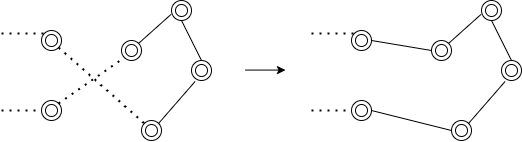
\includegraphics[scale=0.7]{grafika/2opt.png}
	\caption{Metoda 2-opt}
	\label{2opt}
\end{figure}	

\subsection{Propozycje optymalizacji}
	Aby rozwa�y� wi�cej tras zwracanych przez algorytmy zach�anne zaproponowano u�ycie wsp�czynnika b��du przy dokonywaniu przez algorytm w danym momencie najlepszego dla niego wyboru. Wsp�czynnik dzia�a na zasadzie brania pod uwag� gorszego wyboru, aby zwi�kszy� liczb� przegl�danych odcink�w. Ma to na celu mo�liwo�� znalezienia lepszego rozwi�zania ni� takiego jakie zwr�ci�by sam algorytm. Wsp�czynnik b��du mo�e by� uruchamiany na ka�dym etapie budowania docelowej trasy. Zastosowanie wsp�czynnika b��du mo�e podnie�� z�o�ono�� algorytmu nawet do $\theta$(\(n^n\)), gdzie $n$ jest r�wne liczbie wierzcho�k�w. St�d propozycj� jest stosowanie wsp�czynnika b��du tylko na wybranych trzech etapach budowania ko�cowej trasy. Pierwszy etap polega� b�dzie na uruchomieniu wsp�czynnika b��du od samego pocz�tku budowania docelowej trasy. Natomiast drugi etap polega� b�dzie na zaaplikowaniu wsp�czynnika b��du dopiero w po�owie procesu tworzenia docelowej trasy. Ostatni etap b�dzie testowa� wsp�czynnik b��du przy finalizowaniu trasy. Parametry u�yte do bada� zosta�y dok�adniej opisane w rozdziale sz�stym.

\chapter{Badania}

\section{Wyniki algorytmu genetycznego}

\section{Wyniki algorytmu mr�wkowego}

\section{Wyniki algorytmu mr�wkowego}

\chapter{Badania}

\section{Trasa I}

\subsection{Wyniki algorytmu genetycznego}

\begin{table}[]
\caption[Trasa I - �rednie wyniki dla algorytmu genetycznego]
{Trasa I - �rednie wyniki algorytmu genetycznego dla danych parametr�w wej�ciowych}
\scalebox{0.8}{
\begin{tabular}{|l|l|l|l|l|l|l|l|l|l|l|}
\hline
\rowcolor[HTML]{C0C0C0} 
\multicolumn{1}{|c|}{\cellcolor[HTML]{C0C0C0}}                    & \multicolumn{1}{c|}{\cellcolor[HTML]{C0C0C0}}                    & PMX                           & PMX                           & PMX                           & OX                            & OX                            & OX                            & CX                            & CX                            & CX                            \\ \cline{3-11} 
\rowcolor[HTML]{C0C0C0} 
\multicolumn{1}{|c|}{\multirow{-2}{*}{\cellcolor[HTML]{C0C0C0}N}} & \multicolumn{1}{c|}{\multirow{-2}{*}{\cellcolor[HTML]{C0C0C0}k}} & Insert                        & Replace                       & Revert                        & Insert                        & Replace                       & Revert                        & Insert                        & Replace                       & Revert                        \\ \hline
\rowcolor[HTML]{FFFFFF} 
\cellcolor[HTML]{C0C0C0}100                                       & \cellcolor[HTML]{C0C0C0}100                                      & {\color[HTML]{333333} 91502}  & 96029                         & 105868                        & 102746                        & 109380                        & 115816                        & 97015                         & 112795                        & 116291                        \\ \hline
\rowcolor[HTML]{FFFFFF} 
\cellcolor[HTML]{C0C0C0}100                                       & \cellcolor[HTML]{C0C0C0}1000                                     & 52959                         & 67241                         & 80988                         & 58800                         & 70722                         & 93124                         & 55599                         & 67370                         & 92538                         \\ \hline
\rowcolor[HTML]{FFFFFF} 
\cellcolor[HTML]{C0C0C0}100                                       & \cellcolor[HTML]{C0C0C0}2000                                     & 49747                         & 61007                         & 80468                         & 52822                         & 64938                         & 89324                         & 51134                         & 61108                         & 86920                         \\ \hline
\rowcolor[HTML]{FFFFFF} 
\cellcolor[HTML]{C0C0C0}100                                       & \cellcolor[HTML]{C0C0C0}4000                                     & 49368                         & 59649                         & 79494                         & 50284                         & 62967                         & 98000                         & \cellcolor[HTML]{FFCB2F}48571 & 57028                         & 85739                         \\ \hline
\rowcolor[HTML]{FFFFFF} 
\cellcolor[HTML]{C0C0C0}1000                                      & \cellcolor[HTML]{C0C0C0}100                                      & 55008                         & 67898                         & 56269                         & 64427                         & 63525                         & 69052                         & {\color[HTML]{333333} 49959}  & 53471                         & 58104                         \\ \hline
\rowcolor[HTML]{FFFC9E} 
\cellcolor[HTML]{C0C0C0}1000                                      & \cellcolor[HTML]{C0C0C0}1000                                     & 37347                         & 42081                         & \cellcolor[HTML]{FFFFFF}49527 & 41809                         & 46600                         & \cellcolor[HTML]{FFFFFF}60650 & \cellcolor[HTML]{FFCB2F}33768 & 37948                         & 50090                         \\ \hline
\rowcolor[HTML]{FFFC9E} 
\cellcolor[HTML]{C0C0C0}1000                                      & \cellcolor[HTML]{C0C0C0}2000                                     & 39158                         & 40581                         & \cellcolor[HTML]{FFFFFF}50985 & 40903                         & 45041                         & \cellcolor[HTML]{FFFFFF}64489 & \cellcolor[HTML]{FFCB2F}33843 & 38791                         & 48072                         \\ \hline
\cellcolor[HTML]{C0C0C0}1000                                      & \cellcolor[HTML]{C0C0C0}4000                                     & \cellcolor[HTML]{FFFC9E}37951 & \cellcolor[HTML]{FFFC9E}42112 & \cellcolor[HTML]{FFFFFF}50359 & \cellcolor[HTML]{FFFC9E}40036 & \cellcolor[HTML]{FFFC9E}47795 & \cellcolor[HTML]{FFFFFF}62245 & \cellcolor[HTML]{FFCB2F}34961 & \cellcolor[HTML]{FFFC9E}37842 & \cellcolor[HTML]{FFFFFF}49857 \\ \hline
\rowcolor[HTML]{FFFFFF} 
\cellcolor[HTML]{C0C0C0}2000                                      & \cellcolor[HTML]{C0C0C0}100                                      & 51624                         & 48902                         & 49112                         & 62336                         & 61150                         & 57542                         & \cellcolor[HTML]{FFCB2F}40969 & \cellcolor[HTML]{FFFC9E}44643 & \cellcolor[HTML]{FFFC9E}42287 \\ \hline
\rowcolor[HTML]{FFFC9E} 
\cellcolor[HTML]{C0C0C0}2000                                      & \cellcolor[HTML]{C0C0C0}1000                                     & 36492                         & 39233                         & 43081                         & 38086                         & 45761                         & \cellcolor[HTML]{FFFFFF}53166 & \cellcolor[HTML]{FFCB2F}32571 & 35453                         & 39076                         \\ \hline
\rowcolor[HTML]{FFFC9E} 
\cellcolor[HTML]{C0C0C0}2000                                      & \cellcolor[HTML]{C0C0C0}2000                                     & 36410                         & 40379                         & 40711                         & 39554                         & 41320                         & \cellcolor[HTML]{FFFFFF}52030 & \cellcolor[HTML]{34FF34}32326 & 35353                         & 40382                         \\ \hline
\rowcolor[HTML]{FFFC9E} 
\cellcolor[HTML]{C0C0C0}2000                                      & \cellcolor[HTML]{C0C0C0}4000                                     & 35406                         & 38159                         & 42454                         & 39145                         & 44137                         & \cellcolor[HTML]{FFFFFF}51350 & \cellcolor[HTML]{FFCB2F}32667 & 34999                         & 48295                         \\ \hline
\end{tabular}}
\end{table}

\begin{table}[]
\caption[Trasa I - najlepsze wyniki dla algorytmu genetycznego]
{Trasa I - najlepsze wyniki algorytmu genetycznego dla danych parametr�w wej�ciowych}
\scalebox{0.8}{
\begin{tabular}{|l|l|l|l|l|l|l|l|l|l|l|}
\hline
\rowcolor[HTML]{C0C0C0} 
\multicolumn{1}{|c|}{\cellcolor[HTML]{C0C0C0}}                    & \multicolumn{1}{c|}{\cellcolor[HTML]{C0C0C0}}                    & PMX                           & PMX                           & PMX                           & OX                            & OX                            & OX                            & CX                                                   & CX                            & CX                            \\ \cline{3-11} 
\rowcolor[HTML]{C0C0C0} 
\multicolumn{1}{|c|}{\multirow{-2}{*}{\cellcolor[HTML]{C0C0C0}N}} & \multicolumn{1}{c|}{\multirow{-2}{*}{\cellcolor[HTML]{C0C0C0}k}} & Insert                        & Swap                          & Revert                        & Insert                        & Swap                          & Revert                        & Insert                                               & Swap                          & Revert                        \\ \hline
\rowcolor[HTML]{FFFFFF} 
\cellcolor[HTML]{C0C0C0}100                                       & \cellcolor[HTML]{C0C0C0}100                                      & 80385                         & 87226                         & 81154                         & 90764                         & 99185                         & 101137                        & 72268                                                & 103408                        & 92859                         \\ \hline
\rowcolor[HTML]{FFFFFF} 
\cellcolor[HTML]{C0C0C0}100                                       & \cellcolor[HTML]{C0C0C0}1000                                     & \cellcolor[HTML]{FFCB2F}45076 & 62481                         & 67443                         & 53948                         & 60699                         & 78382                         & \cellcolor[HTML]{FFFC9E}45134                        & 56918                         & 79955                         \\ \hline
\rowcolor[HTML]{FFFFFF} 
\cellcolor[HTML]{C0C0C0}100                                       & \cellcolor[HTML]{C0C0C0}2000                                     & \cellcolor[HTML]{FFCB2F}40964 & 53316                         & 70100                         & 45500                         & 55396                         & 80719                         & \cellcolor[HTML]{FFFC9E}43142                        & 54430                         & 79636                         \\ \hline
\rowcolor[HTML]{FFFFFF} 
\cellcolor[HTML]{C0C0C0}100                                       & \cellcolor[HTML]{C0C0C0}4000                                     & \cellcolor[HTML]{FFFC9E}44853 & 52397                         & 69287                         & 40628                         & 56153                         & 91440                         & \cellcolor[HTML]{FFCB2F}41805                        & \cellcolor[HTML]{FFFC9E}45953 & 72035                         \\ \hline
\cellcolor[HTML]{C0C0C0}1000                                      & \cellcolor[HTML]{C0C0C0}100                                      & \cellcolor[HTML]{FFFC9E}45769 & \cellcolor[HTML]{FFFFFF}59523 & \cellcolor[HTML]{FFFFFF}50232 & \cellcolor[HTML]{FFFFFF}56634 & \cellcolor[HTML]{FFFFFF}58272 & \cellcolor[HTML]{FFFFFF}62965 & \cellcolor[HTML]{FFCB2F}{\color[HTML]{333333} 40804} & \cellcolor[HTML]{FFFC9E}42391 & \cellcolor[HTML]{FFFC9E}41647 \\ \hline
\rowcolor[HTML]{FFFC9E} 
\cellcolor[HTML]{C0C0C0}1000                                      & \cellcolor[HTML]{C0C0C0}1000                                     & 34630                         & 36034                         & 42016                         & 39283                         & 44320                         & \cellcolor[HTML]{FFFFFF}53480 & \cellcolor[HTML]{FFCC67}32433                        & 35227                         & 37569                         \\ \hline
\rowcolor[HTML]{FFFC9E} 
\cellcolor[HTML]{C0C0C0}1000                                      & \cellcolor[HTML]{C0C0C0}2000                                     & 35051                         & 36704                         & 45852                         & 35709                         & 41317                         & \cellcolor[HTML]{FFFFFF}57478 & \cellcolor[HTML]{FFCB2F}32334                        & 35576                         & 39953                         \\ \hline
\rowcolor[HTML]{FFFC9E} 
\cellcolor[HTML]{C0C0C0}1000                                      & \cellcolor[HTML]{C0C0C0}4000                                     & 33268                         & 37649                         & 44333                         & 35718                         & 41883                         & 49322                         & \cellcolor[HTML]{FFCB2F}33089                        & 34642                         & 40220                         \\ \hline
\rowcolor[HTML]{FFFC9E} 
\cellcolor[HTML]{C0C0C0}2000                                      & \cellcolor[HTML]{C0C0C0}100                                      & 44493                         & 42497                         & 42138                         & 56466                         & 56884                         & \cellcolor[HTML]{FFFFFF}52010 & \cellcolor[HTML]{FFCB2F}36349                        & 38830                         & 38461                         \\ \hline
\rowcolor[HTML]{FFFC9E} 
\cellcolor[HTML]{C0C0C0}2000                                      & \cellcolor[HTML]{C0C0C0}1000                                     & 33609                         & 36100                         & 37047                         & 34801                         & 38625                         & 40817                         & \cellcolor[HTML]{34FF34}30939                        & 33284                         & 36203                         \\ \hline
\rowcolor[HTML]{FFFC9E} 
\cellcolor[HTML]{C0C0C0}2000                                      & \cellcolor[HTML]{C0C0C0}2000                                     & 33257                         & 36216                         & 37967                         & 34591                         & 36458                         & 47022                         & \cellcolor[HTML]{FFCB2F}31118                        & 32798                         & 36203                         \\ \hline
\rowcolor[HTML]{FFFC9E} 
\cellcolor[HTML]{C0C0C0}2000                                      & \cellcolor[HTML]{C0C0C0}4000                                     & 31347                         & 36834                         & 40193                         & 34269                         & 37693                         & 43242                         & \cellcolor[HTML]{FFCB2F}31118                        & 33245                         & 35271                         \\ \hline
\end{tabular}}
\end{table}

\begin{figure}[h]
	\centering
	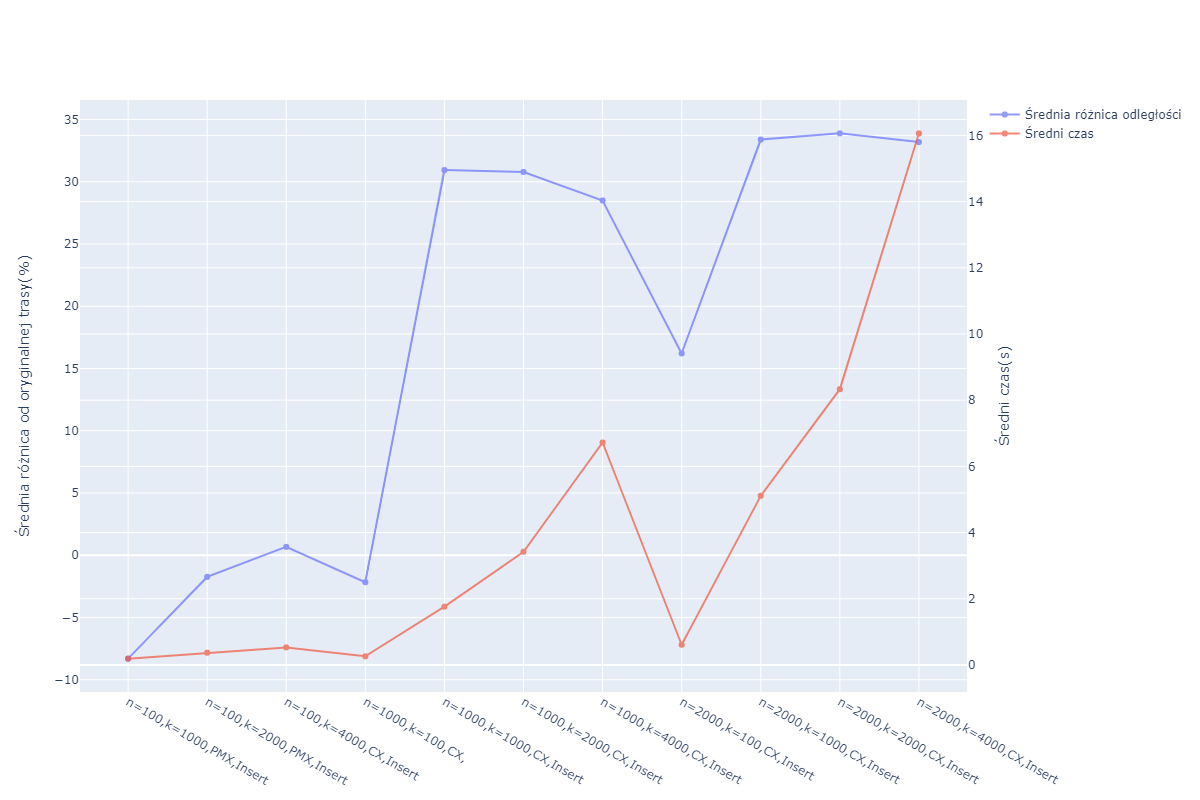
\includegraphics[scale=0.4]{grafika/Trasa1GA.png}
	\caption{Trasa I - Zale�no�� �redniej odleg�o�ci od czasu}
	\label{mutacja}
\end{figure}	

\subsection{Wyniki algorytmu mr�wkowego}

\subsection{Wyniki algorytm�w zach�annych}

\subsection{Por�wnanie algorytm�w}

\section{Trasa II}
\subsection{Wyniki algorytmu genetycznego}
\begin{table}[htb]
\caption[Trasa II -�rednie wyniki dla algorytmu genetycznego]
{Trasa II - �rednie wyniki algorytmu genetycznego dla danych parametr�w wej�ciowych}
\scalebox{0.8}{
\begin{tabular}{|l|l|l|l|l|l|l|l|l|l|l|}
\hline
\rowcolor[HTML]{C0C0C0} 
\multicolumn{1}{|c|}{\cellcolor[HTML]{C0C0C0}}                    & \multicolumn{1}{c|}{\cellcolor[HTML]{C0C0C0}}                    & \multicolumn{1}{c|}{\cellcolor[HTML]{C0C0C0}PMX}    & \multicolumn{1}{c|}{\cellcolor[HTML]{C0C0C0}PMX}     & \multicolumn{1}{c|}{\cellcolor[HTML]{C0C0C0}PMX}    & \multicolumn{1}{c|}{\cellcolor[HTML]{C0C0C0}OX}     & \multicolumn{1}{c|}{\cellcolor[HTML]{C0C0C0}OX}      & \multicolumn{1}{c|}{\cellcolor[HTML]{C0C0C0}OX}     & \multicolumn{1}{c|}{\cellcolor[HTML]{C0C0C0}CX}     & \multicolumn{1}{c|}{\cellcolor[HTML]{C0C0C0}CX}      & \multicolumn{1}{c|}{\cellcolor[HTML]{C0C0C0}CX}     \\ \cline{3-11} 
\rowcolor[HTML]{C0C0C0} 
\multicolumn{1}{|c|}{\multirow{-2}{*}{\cellcolor[HTML]{C0C0C0}N}} & \multicolumn{1}{c|}{\multirow{-2}{*}{\cellcolor[HTML]{C0C0C0}k}} & \multicolumn{1}{c|}{\cellcolor[HTML]{C0C0C0}Insert} & \multicolumn{1}{c|}{\cellcolor[HTML]{C0C0C0}Replace} & \multicolumn{1}{c|}{\cellcolor[HTML]{C0C0C0}Revert} & \multicolumn{1}{c|}{\cellcolor[HTML]{C0C0C0}Insert} & \multicolumn{1}{c|}{\cellcolor[HTML]{C0C0C0}Replace} & \multicolumn{1}{c|}{\cellcolor[HTML]{C0C0C0}Revert} & \multicolumn{1}{c|}{\cellcolor[HTML]{C0C0C0}Insert} & \multicolumn{1}{c|}{\cellcolor[HTML]{C0C0C0}Replace} & \multicolumn{1}{c|}{\cellcolor[HTML]{C0C0C0}Revert} \\ \hline
\rowcolor[HTML]{FFFFFF} 
\cellcolor[HTML]{C0C0C0}100                                       & \cellcolor[HTML]{C0C0C0}100                                      & {\color[HTML]{333333} 99575}                        & 107771                                               & 111797                                              & 113364                                              & 119707                                               & 120570                                              & 110318                                              & 116843                                               & 116749                                              \\ \hline
\rowcolor[HTML]{FFFFFF} 
\cellcolor[HTML]{C0C0C0}100                                       & \cellcolor[HTML]{C0C0C0}1000                                     & 56105                                               & 70104                                                & 88449                                               & 60788                                               & 71531                                                & 93290                                               & 59452                                               & 70589                                                & 88734                                               \\ \hline
\rowcolor[HTML]{FFFFFF} 
\cellcolor[HTML]{C0C0C0}100                                       & \cellcolor[HTML]{C0C0C0}2000                                     & 48407                                               & 61102                                                & 87698                                               & 50719                                               & 61516                                                & 92912                                               & 48634                                               & 61984                                                & 88546                                               \\ \hline
\rowcolor[HTML]{FFFFFF} 
\cellcolor[HTML]{C0C0C0}100                                       & \cellcolor[HTML]{C0C0C0}4000                                     & 47154                                               & 54452                                                & 47154                                               & 48203                                               & 55866                                                & 92145                                               & 43488                                               & 52586                                                & 86276                                               \\ \hline
\rowcolor[HTML]{FFFFFF} 
\cellcolor[HTML]{C0C0C0}1000                                      & \cellcolor[HTML]{C0C0C0}100                                      & 65248                                               & 67898                                                & 64703                                               & 78946                                               & 83318                                                & 81904                                               & {\color[HTML]{333333} 47854}                        & 46921                                                & 49695                                               \\ \hline
\rowcolor[HTML]{FFFFFF} 
\cellcolor[HTML]{C0C0C0}1000                                      & \cellcolor[HTML]{C0C0C0}1000                                     & \cellcolor[HTML]{FFFC9E}39419                       & 43935                                                & 55085                                               & 41294                                               & 46914                                                & 68463                                               & \cellcolor[HTML]{FFCB2F}30385                       & \cellcolor[HTML]{FFFC9E}32616                        & 43041                                               \\ \hline
\cellcolor[HTML]{C0C0C0}1000                                      & \cellcolor[HTML]{C0C0C0}2000                                     & \cellcolor[HTML]{FFFC9E}34882                       & \cellcolor[HTML]{FFFFFF}40914                        & \cellcolor[HTML]{FFFFFF}57467                       & \cellcolor[HTML]{FFFC9E}39237                       & \cellcolor[HTML]{FFFFFF}44605                        & \cellcolor[HTML]{FFFFFF}65532                       & \cellcolor[HTML]{FFCB2F}30631                       & \cellcolor[HTML]{FFFC9E}31273                        & \cellcolor[HTML]{FFFFFF}48346                       \\ \hline
\cellcolor[HTML]{C0C0C0}1000                                      & \cellcolor[HTML]{C0C0C0}4000                                     & \cellcolor[HTML]{FFFC9E}36160                       & \cellcolor[HTML]{FFFC9E}39848                        & \cellcolor[HTML]{FFFFFF}55774                       & \cellcolor[HTML]{FFFC9E}36414                       & \cellcolor[HTML]{FFFFFF}44856                        & \cellcolor[HTML]{FFFFFF}68215                       & \cellcolor[HTML]{FFCB2F}30443                       & \cellcolor[HTML]{FFFC9E}30720                        & \cellcolor[HTML]{FFFFFF}48295                       \\ \hline
\rowcolor[HTML]{FFFFFF} 
\cellcolor[HTML]{C0C0C0}2000                                      & \cellcolor[HTML]{C0C0C0}100                                      & 58533                                               & 59876                                                & 60898                                               & 70291                                               & 71693                                                & 72095                                               & \cellcolor[HTML]{FFFC9E}38655                       & \cellcolor[HTML]{FFFC9E}39129                        & \cellcolor[HTML]{FFCB2F}37204                       \\ \hline
\cellcolor[HTML]{C0C0C0}2000                                      & \cellcolor[HTML]{C0C0C0}1000                                     & \cellcolor[HTML]{FFFC9E}34939                       & \cellcolor[HTML]{FFFC9E}38272                        & \cellcolor[HTML]{FFFFFF}49381                       & \cellcolor[HTML]{FFFC9E}35951                       & \cellcolor[HTML]{FFFC9E}39779                        & \cellcolor[HTML]{FFFFFF}62656                       & \cellcolor[HTML]{34FF34}28196                       & \cellcolor[HTML]{FFFFFF}29415                        & \cellcolor[HTML]{FFFFFF}33519                       \\ \hline
\cellcolor[HTML]{C0C0C0}2000                                      & \cellcolor[HTML]{C0C0C0}2000                                     & \cellcolor[HTML]{FFFC9E}32900                       & \cellcolor[HTML]{FFFC9E}39068                        & \cellcolor[HTML]{FFFFFF}48607                       & \cellcolor[HTML]{FFFC9E}34474                       & \cellcolor[HTML]{FFFFFF}41349                        & \cellcolor[HTML]{FFFFFF}56907                       & \cellcolor[HTML]{FFFC9E}28802                       & \cellcolor[HTML]{FFCB2F}28506                        & \cellcolor[HTML]{FFFC9E}34458                       \\ \hline
\rowcolor[HTML]{FFFC9E} 
\cellcolor[HTML]{C0C0C0}2000                                      & \cellcolor[HTML]{C0C0C0}4000                                     & 32626                                               & 36244                                                & \cellcolor[HTML]{FFFFFF}49132                       & 36333                                               & 39164                                                & \cellcolor[HTML]{FFFFFF}57952                       & 28808                                               & \cellcolor[HTML]{FFCB2F}28453                        & 32683                                               \\ \hline
\end{tabular}}
\end{table}


\begin{table}[]
\caption[Trasa II - najlepsze wyniki dla algorytmu genetycznego]
{Trasa II - najlepsze wyniki algorytmu genetycznego dla danych parametr�w wej�ciowych}
\scalebox{0.8}{
\begin{tabular}{|l|l|l|l|l|l|l|l|l|l|l|}
\hline
\rowcolor[HTML]{C0C0C0} 
\multicolumn{1}{|c|}{\cellcolor[HTML]{C0C0C0}}                    & \multicolumn{1}{c|}{\cellcolor[HTML]{C0C0C0}}                    & PMX                           & PMX                           & PMX                           & OX                            & OX                            & OX                            & CX                                                   & CX                            & CX                            \\ \cline{3-11} 
\rowcolor[HTML]{C0C0C0} 
\multicolumn{1}{|c|}{\multirow{-2}{*}{\cellcolor[HTML]{C0C0C0}N}} & \multicolumn{1}{c|}{\multirow{-2}{*}{\cellcolor[HTML]{C0C0C0}k}} & Insert                        & Replace                       & Revert                        & Insert                        & Replace                       & Revert                        & Insert                                               & Replace                       & Revert                        \\ \hline
\rowcolor[HTML]{FFFFFF} 
\cellcolor[HTML]{C0C0C0}100                                       & \cellcolor[HTML]{C0C0C0}100                                      & {\color[HTML]{333333} 89707}  & 95824                         & 100856                        & 102788                        & 110057                        & 114491                        & 104749                                               & 104765                        & 101883                        \\ \hline
\rowcolor[HTML]{FFFFFF} 
\cellcolor[HTML]{C0C0C0}100                                       & \cellcolor[HTML]{C0C0C0}1000                                     & 44863                         & 63868                         & 76641                         & 54433                         & 59588                         & 80783                         & 53688                                                & 55723                         & 75815                         \\ \hline
\rowcolor[HTML]{FFFFFF} 
\cellcolor[HTML]{C0C0C0}100                                       & \cellcolor[HTML]{C0C0C0}2000                                     & 42084                         & 56000                         & 79817                         & 46908                         & 54427                         & 86609                         & 43440                                                & 48834                         & 80426                         \\ \hline
\rowcolor[HTML]{FFFFFF} 
\cellcolor[HTML]{C0C0C0}100                                       & \cellcolor[HTML]{C0C0C0}4000                                     & \cellcolor[HTML]{FFFC9E}40309 & 49246                         & 40309                         & 43816                         & 49864                         & 78281                         & \cellcolor[HTML]{FFCB2F}37172                        & 47158                         & 78780                         \\ \hline
\rowcolor[HTML]{FFFFFF} 
\cellcolor[HTML]{C0C0C0}1000                                      & \cellcolor[HTML]{C0C0C0}100                                      & 53565                         & 59523                         & 59419                         & 71181                         & 75567                         & 73827                         & \cellcolor[HTML]{FFFC9E}{\color[HTML]{333333} 40068} & \cellcolor[HTML]{FFFC9E}38220 & \cellcolor[HTML]{FFCB2F}33442 \\ \hline
\cellcolor[HTML]{C0C0C0}1000                                      & \cellcolor[HTML]{C0C0C0}1000                                     & \cellcolor[HTML]{FFFC9E}34352 & \cellcolor[HTML]{FFFC9E}38069 & \cellcolor[HTML]{FFFFFF}48381 & \cellcolor[HTML]{FFFC9E}34282 & \cellcolor[HTML]{FFFFFF}44087 & \cellcolor[HTML]{FFFFFF}62194 & \cellcolor[HTML]{FFCB2F}28947                        & \cellcolor[HTML]{FFFC9E}29655 & \cellcolor[HTML]{FFFC9E}34089 \\ \hline
\cellcolor[HTML]{C0C0C0}1000                                      & \cellcolor[HTML]{C0C0C0}2000                                     & \cellcolor[HTML]{FFFC9E}32942 & \cellcolor[HTML]{FFFC9E}36491 & \cellcolor[HTML]{FFFFFF}48353 & \cellcolor[HTML]{FFFC9E}33013 & \cellcolor[HTML]{FFFFFF}40481 & \cellcolor[HTML]{FFFFFF}58856 & \cellcolor[HTML]{FFFC9E}28047                        & \cellcolor[HTML]{FFCB2F}27858 & \cellcolor[HTML]{FFFC9E}35650 \\ \hline
\rowcolor[HTML]{FFFC9E} 
\cellcolor[HTML]{C0C0C0}1000                                      & \cellcolor[HTML]{C0C0C0}4000                                     & 33021                         & 33720                         & \cellcolor[HTML]{FFFFFF}47438 & 29602                         & 38640                         & \cellcolor[HTML]{FFFFFF}57355 & 28442                                                & \cellcolor[HTML]{FFCB2F}28027 & 35271                         \\ \hline
\rowcolor[HTML]{FFFFFF} 
\cellcolor[HTML]{C0C0C0}2000                                      & \cellcolor[HTML]{C0C0C0}100                                      & 50007                         & 53464                         & 51193                         & 61228                         & 67171                         & 59619                         & \cellcolor[HTML]{FFFC9E}33775                        & \cellcolor[HTML]{FFFC9E}35063 & \cellcolor[HTML]{FFCB2F}31852 \\ \hline
\rowcolor[HTML]{FFFC9E} 
\cellcolor[HTML]{C0C0C0}2000                                      & \cellcolor[HTML]{C0C0C0}1000                                     & 29758                         & 33420                         & \cellcolor[HTML]{FFFFFF}43562 & 32178                         & 33255                         & \cellcolor[HTML]{FFFFFF}56070 & \cellcolor[HTML]{34FF34}27655                        & 27910                         & 29839                         \\ \hline
\rowcolor[HTML]{FFFC9E} 
\cellcolor[HTML]{C0C0C0}2000                                      & \cellcolor[HTML]{C0C0C0}2000                                     & 31390                         & 35329                         & 38151                         & 30047                         & 31229                         & \cellcolor[HTML]{FFFFFF}48944 & 28178                                                & \cellcolor[HTML]{FFCB2F}27381 & 29839                         \\ \hline
\rowcolor[HTML]{FFFC9E} 
\cellcolor[HTML]{C0C0C0}2000                                      & \cellcolor[HTML]{C0C0C0}4000                                     & 30080                         & 31724                         & 38944                         & 32360                         & 35025                         & \cellcolor[HTML]{FFFFFF}49517 & 28177                                                & \cellcolor[HTML]{FFCB2F}27925 & 29840                         \\ \hline
\end{tabular}}
\end{table}

\begin{figure}[h]
	\centering
	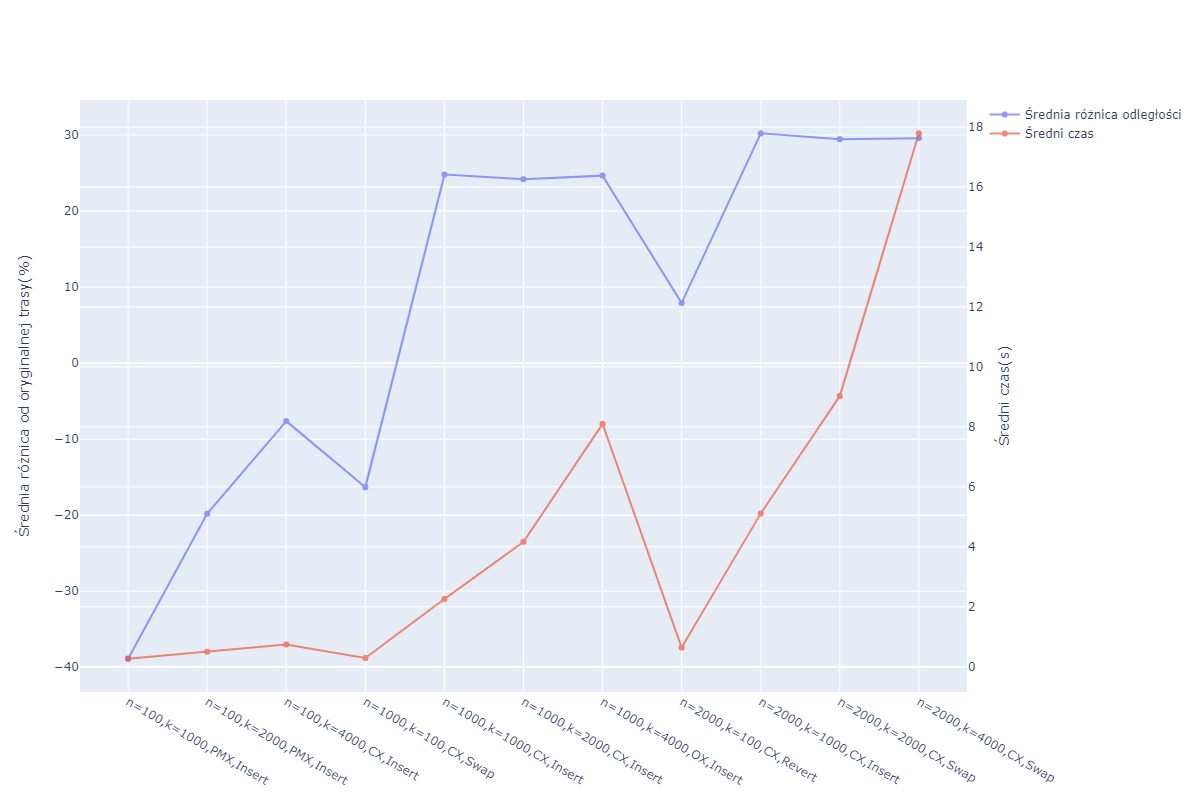
\includegraphics[scale=0.4]{grafika/Trasa2GA.png}
	\caption{Trasa II - Zale�no�� �redniej odleg�o�ci od czasu}
	\label{mutacja}
\end{figure}	

\subsection{Wyniki algorytmu mr�wkowego}

\subsection{Wyniki algorytm�w zach�annych}

\subsection{Por�wnanie algorytm�w}

\section{Trasa III}

\subsection{Wyniki algorytmu genetycznego}

% Please add the following required packages to your document preamble:
% \usepackage{multirow}
% \usepackage[table,xcdraw]{xcolor}
% If you use beamer only pass "xcolor=table" option, i.e. \documentclass[xcolor=table]{beamer}
\begin{table}[]
\caption[Trasa III -�rednie wyniki dla algorytmu genetycznego]
{Trasa III - �rednie wyniki algorytmu genetycznego dla danych parametr�w wej�ciowych}
\scalebox{0.8}{
\begin{tabular}{|l|l|l|l|l|l|l|l|l|l|l|}
\hline
\rowcolor[HTML]{C0C0C0} 
\multicolumn{1}{|c|}{\cellcolor[HTML]{C0C0C0}}                    & \multicolumn{1}{c|}{\cellcolor[HTML]{C0C0C0}}                    & PMX                           & PMX    & PMX    & OX     & OX     & OX     & CX                            & CX                            & CX     \\ \cline{3-11} 
\rowcolor[HTML]{C0C0C0} 
\multicolumn{1}{|c|}{\multirow{-2}{*}{\cellcolor[HTML]{C0C0C0}N}} & \multicolumn{1}{c|}{\multirow{-2}{*}{\cellcolor[HTML]{C0C0C0}k}} & Insert                        & Swap   & Revert & Insert & Swap   & Revert & Insert                        & Swap                          & Revert \\ \hline
\rowcolor[HTML]{FFFFFF} 
\cellcolor[HTML]{C0C0C0}100                                       & \cellcolor[HTML]{C0C0C0}100                                      & 202200                        & 215800 & 223134 & 226673 & 238350 & 244471 & 226996                        & 238909                        & 248130 \\ \hline
\rowcolor[HTML]{FFFFFF} 
\cellcolor[HTML]{C0C0C0}100                                       & \cellcolor[HTML]{C0C0C0}1000                                     & 101445                        & 119726 & 156991 & 108762 & 130635 & 168963 & 121076                        & 140420                        & 170028 \\ \hline
\rowcolor[HTML]{FFFFFF} 
\cellcolor[HTML]{C0C0C0}100                                       & \cellcolor[HTML]{C0C0C0}2000                                     & 88501                         & 112378 & 149298 & 95249  & 112897 & 159348 & 95405                         & 110801                        & 162912 \\ \hline
\rowcolor[HTML]{FFFFFF} 
\cellcolor[HTML]{C0C0C0}100                                       & \cellcolor[HTML]{C0C0C0}4000                                     & 81056                         & 97882  & 151635 & 80120  & 99671  & 163374 & 74624                         & 97972                         & 153400 \\ \hline
\rowcolor[HTML]{FFFFFF} 
\cellcolor[HTML]{C0C0C0}1000                                      & \cellcolor[HTML]{C0C0C0}100                                      & 138988                        & 141411 & 138102 & 159437 & 165202 & 161127 & {\color[HTML]{333333} 100709} & 114035                        & 108668 \\ \hline
\rowcolor[HTML]{FFFFFF} 
\cellcolor[HTML]{C0C0C0}1000                                      & \cellcolor[HTML]{C0C0C0}1000                                     & 60548                         & 66745  & 93017  & 70666  & 76984  & 117566 & \cellcolor[HTML]{FFCB2F}43728 & 54573                         & 85516  \\ \hline
\rowcolor[HTML]{FFFFFF} 
\cellcolor[HTML]{C0C0C0}1000                                      & \cellcolor[HTML]{C0C0C0}2000                                     & 53736                         & 68402  & 96311  & 59332  & 71183  & 117932 & \cellcolor[HTML]{FFCB2F}42545 & \cellcolor[HTML]{FFFC9E}50305 & 90144  \\ \hline
\rowcolor[HTML]{FFFFFF} 
\cellcolor[HTML]{C0C0C0}1000                                      & \cellcolor[HTML]{C0C0C0}4000                                     & \cellcolor[HTML]{FFFC9E}49323 & 66474  & 96935  & 56877  & 69448  & 118314 & \cellcolor[HTML]{FFCB2F}40121 & \cellcolor[HTML]{FFFC9E}48213 & 86232  \\ \hline
\rowcolor[HTML]{FFFFFF} 
\cellcolor[HTML]{C0C0C0}2000                                      & \cellcolor[HTML]{C0C0C0}100                                      & 126626                        & 127066 & 125408 & 147299 & 148430 & 147276 & 64776                         & 89803                         & 81523  \\ \hline
\rowcolor[HTML]{FFFFFF} 
\cellcolor[HTML]{C0C0C0}2000                                      & \cellcolor[HTML]{C0C0C0}1000                                     & 54123                         & 64199  & 82598  & 57743  & 68314  & 103521 & \cellcolor[HTML]{FFCB2F}34365 & \cellcolor[HTML]{FFFC9E}39530 & 50624  \\ \hline
\rowcolor[HTML]{FFFFFF} 
\cellcolor[HTML]{C0C0C0}2000                                      & \cellcolor[HTML]{C0C0C0}2000                                     & \cellcolor[HTML]{FFFC9E}45893 & 55922  & 82523  & 51700  & 63697  & 96266  & \cellcolor[HTML]{FFCB2F}36518 & \cellcolor[HTML]{FFFC9E}39200 & 59014  \\ \hline
\rowcolor[HTML]{FFFFFF} 
\cellcolor[HTML]{C0C0C0}2000                                      & \cellcolor[HTML]{C0C0C0}4000                                     & \cellcolor[HTML]{FFFC9E}47206 & 57436  & 81653  & 53149  & 66321  & 96440  & \cellcolor[HTML]{34FF34}34168 & \cellcolor[HTML]{FFFC9E}37951 & 56645  \\ \hline
\end{tabular}}
\end{table}

\begin{table}[]
\caption[Trasa III - najlepsze wyniki dla algorytmu genetycznego]
{Trasa III - najlepsze wyniki algorytmu genetycznego dla danych parametr�w wej�ciowych}
\scalebox{0.8}{
\begin{tabular}{|
>{\columncolor[HTML]{C0C0C0}}l |
>{\columncolor[HTML]{C0C0C0}}l |
>{\columncolor[HTML]{FFFFFF}}l |
>{\columncolor[HTML]{FFFFFF}}l |
>{\columncolor[HTML]{FFFFFF}}l |
>{\columncolor[HTML]{FFFFFF}}l |
>{\columncolor[HTML]{FFFFFF}}l |
>{\columncolor[HTML]{FFFFFF}}l |l|l|
>{\columncolor[HTML]{FFFFFF}}l |}
\hline
\multicolumn{1}{|c|}{\cellcolor[HTML]{C0C0C0}}                    & \multicolumn{1}{c|}{\cellcolor[HTML]{C0C0C0}}                    & \cellcolor[HTML]{C0C0C0}PMX    & \cellcolor[HTML]{C0C0C0}PMX   & \cellcolor[HTML]{C0C0C0}PMX    & \cellcolor[HTML]{C0C0C0}OX     & \cellcolor[HTML]{C0C0C0}OX    & \cellcolor[HTML]{C0C0C0}OX     & \cellcolor[HTML]{C0C0C0}CX                           & \cellcolor[HTML]{C0C0C0}CX     & \cellcolor[HTML]{C0C0C0}CX     \\ \cline{3-11} 
\multicolumn{1}{|c|}{\multirow{-2}{*}{\cellcolor[HTML]{C0C0C0}N}} & \multicolumn{1}{c|}{\multirow{-2}{*}{\cellcolor[HTML]{C0C0C0}k}} & \cellcolor[HTML]{C0C0C0}Insert & \cellcolor[HTML]{C0C0C0}Swap  & \cellcolor[HTML]{C0C0C0}Revert & \cellcolor[HTML]{C0C0C0}Insert & \cellcolor[HTML]{C0C0C0}Swap  & \cellcolor[HTML]{C0C0C0}Revert & \cellcolor[HTML]{C0C0C0}Insert                       & \cellcolor[HTML]{C0C0C0}Swap   & \cellcolor[HTML]{C0C0C0}Revert \\ \hline
\cellcolor[HTML]{C0C0C0}100                                       & \cellcolor[HTML]{C0C0C0}100                                      & 178235                         & 179169                        & 210255                         & 214392                         & 220255                        & 225128                         & \cellcolor[HTML]{FFFFFF}199164                       & \cellcolor[HTML]{FFFFFF}209900 & 228851                         \\ \hline
100                                                               & 1000                                                             & 92035                          & 97541                         & 145836                         & 92447                          & 119218                        & 156940                         & \cellcolor[HTML]{FFFFFF}108633                       & \cellcolor[HTML]{FFFFFF}134528 & 147851                         \\ \hline
100                                                               & 2000                                                             & 75472                          & 99019                         & 133028                         & 82103                          & 100138                        & 150643                         & \cellcolor[HTML]{FFFFFF}82086                        & \cellcolor[HTML]{FFFFFF}100030 & 146323                         \\ \hline
100                                                               & 4000                                                             & 66386                          & 84653                         & 128228                         & 67843                          & 87629                         & 150569                         & \cellcolor[HTML]{FFFFFF}64530                        & \cellcolor[HTML]{FFFFFF}85814  & 128407                         \\ \hline
1000                                                              & 100                                                              & 130408                         & 129829                        & 113771                         & 146677                         & 146199                        & 146851                         & \cellcolor[HTML]{FFFFFF}{\color[HTML]{333333} 80069} & \cellcolor[HTML]{FFFFFF}80657  & 91467                          \\ \hline
1000                                                              & 1000                                                             & 54442                          & 57812                         & 79987                          & 65279                          & 70631                         & 98505                          & \cellcolor[HTML]{FFCB2F}37536                        & \cellcolor[HTML]{FFFC9E}44330  & 70152                          \\ \hline
1000                                                              & 2000                                                             & \cellcolor[HTML]{FFFC9E}43708  & 57296                         & 67415                          & \cellcolor[HTML]{FFFC9E}51213  & 57795                         & 97761                          & \cellcolor[HTML]{FFCB2F}36381                        & \cellcolor[HTML]{FFFFC7}39559  & 64270                          \\ \hline
1000                                                              & 4000                                                             & \cellcolor[HTML]{FFFC9E}43938  & 57678                         & 81284                          & \cellcolor[HTML]{FFFC9E}47695  & 60624                         & 102346                         & \cellcolor[HTML]{FFCB2F}34365                        & \cellcolor[HTML]{FFFFC7}38618  & 69499                          \\ \hline
2000                                                              & 100                                                              & 117579                         & 114351                        & 112117                         & 133323                         & 133203                        & 140060                         & \cellcolor[HTML]{FFFFFF}58239                        & \cellcolor[HTML]{FFFFFF}66450  & 64827                          \\ \hline
2000                                                              & 1000                                                             & \cellcolor[HTML]{FFFC9E}46490  & \cellcolor[HTML]{FFFC9E}47507 & 72252                          & \cellcolor[HTML]{FFFC9E}50359  & 60606                         & 91474                          & \cellcolor[HTML]{34FF34}32374                        & \cellcolor[HTML]{FFFC9E}33408  & \cellcolor[HTML]{FFFC9E}41138  \\ \hline
2000                                                              & 2000                                                             & \cellcolor[HTML]{FFFC9E}42326  & \cellcolor[HTML]{FFFC9E}44568 & 70413                          & \cellcolor[HTML]{FFFC9E}45282  & \cellcolor[HTML]{FFFC9E}53114 & 81577                          & \cellcolor[HTML]{FFCB2F}33070                        & \cellcolor[HTML]{FFFC9E}36492  & \cellcolor[HTML]{FFFC9E}41724  \\ \hline
2000                                                              & 4000                                                             & \cellcolor[HTML]{FFFC9E}43332  & \cellcolor[HTML]{FFFC9E}49969 & 69794                          & \cellcolor[HTML]{FFFC9E}46970  & 56971                         & 83286                          & \cellcolor[HTML]{FFCB2F}32478                        & \cellcolor[HTML]{FFFC9E}33962  & \cellcolor[HTML]{FFFC9E}41975  \\ \hline
\end{tabular}}
\end{table}

\begin{figure}[h]
	\centering
	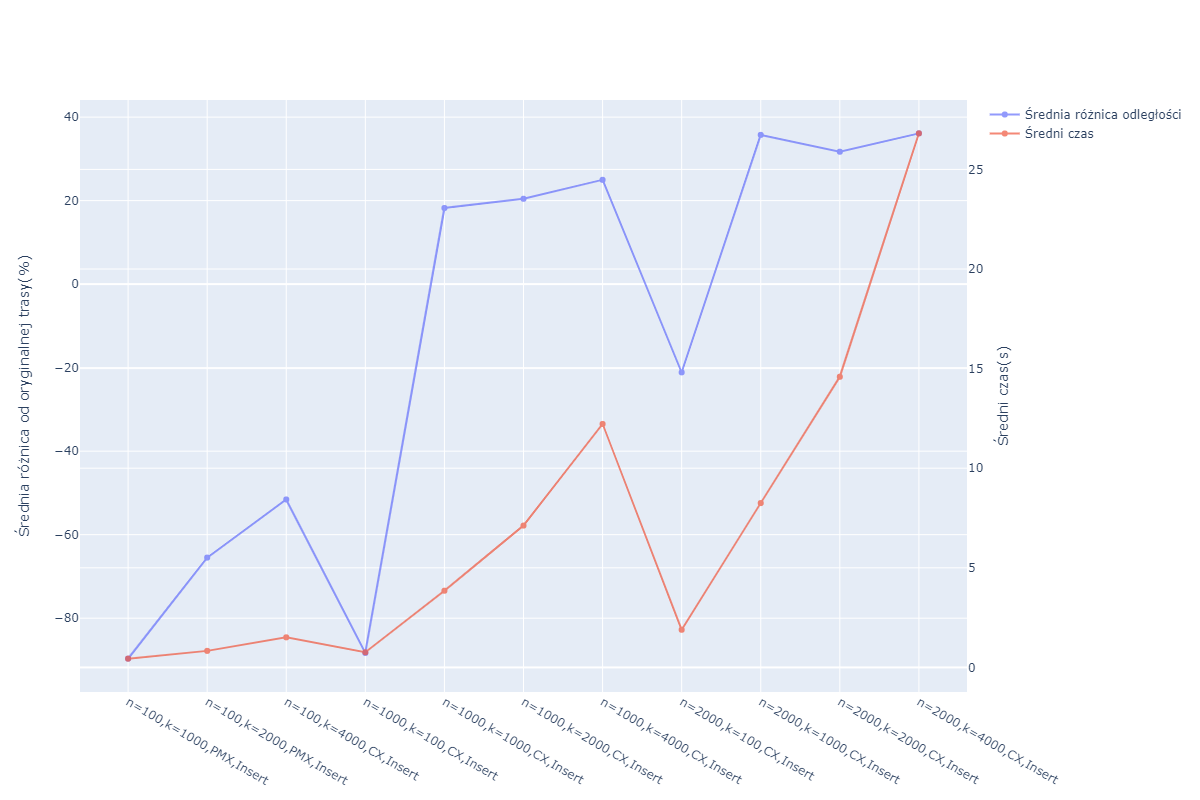
\includegraphics[scale=0.4]{grafika/Trasa3GA.png}
	\caption{Trasa III - Zale�no�� �redniej odleg�o�ci od czasu}
	\label{mutacja}
\end{figure}	

\subsection{Wyniki algorytmu mr�wkowego}

\subsection{Wyniki algorytm�w zach�annych}

\subsection{Por�wnanie algorytm�w}
\chapter*{Podsumowanie -- KL, PN, PS}
\addcontentsline{toc}{chapter}{Podsumowanie}

Cel pracy zosta� osi�gni�ty, wykonana zosta�a optymalizacja tras przejazdu ci�ar�wek z odpadami komunalnymi. Wykorzystane rozwi�zania s� dedykowane do prac nad optymalizacj� problemu komiwoja�era. Dla ka�dego z algorytm�w nale�a�o znale�� takie parametry wej�ciowe, aby optymalizacje d�ugo�ci tras by�y jak najlepsze.

Dzi�ki wykorzystaniu realnych danych do optymalizacji �cie�ek przejazd�w ci�ar�wek z odpadami komunalnymi mo�na zbada� oraz zaproponowa� rozwi�zanie problemu. Dane te zosta�y udost�pnione przez miasto Bia�ystok i wymaga�y odpowiedniego przetworzenia, w celu przeprowadzenia bada�. Wybrane �cie�ki stanowi� faktyczne trasy jakie by�y przebywane. Wybrane trzy losowo trasy sk�ada�y si� odpowiednio z 111, 150 oraz 248 punkt�w. Dzi�ki udost�pnionym rozwi�zaniu przez firm� Google, zosta�y wyliczone rzeczywiste odleg�o�ci pomi�dzy wszystkimi punktami.

Do optymalizacji wybrane zosta�y algorytmy reprezentuj�ce trzy r�ne podej�cia. Algorytm genetyczny, kt�ry zosta� opisany i zbadany przez Paw�a Stypu�kowskiego. Kolejnym algorytmem wybranym by� algorytm mr�wkowy autorstwa Kamila ��towskiego. Jako ostatnie zosta�o zaproponowanych kilka algorytm�w zach�annych przez Przemys�awa Noskowicza.

Algorytm genetyczny oraz mr�wkowy dla ka�dej mo�liwej konfiguracji parametr�w wej�ciowych zosta� uruchomiony dziesi�� razy. Algorytm genetyczny zosta� zbadany dla trzech populacji $N$: 100, 1000 oraz 2000; czterech r�nych warto�ci iteracji $k$: 100, 1000, 2000 oraz 4000; trzech r�nych krzy�owa�: $PMX$, $OX$ oraz $CX$; trzech r�nych mutacji: $Reverse$, $Swap$ oraz $Insert$. Wykonanie wszystkich bada� dla jednej trasy trwa�o kilka godzin. W algorytmie mr�wkowym parametrami wej�ciowymi by�a liczba iteracji oraz wsp�czynnik parowania feromon�w. Wykonanych by�o 50, 75 lub 100 iteracji a wsp�czynnik zakresu by� rozpoczyna� si� od 0.1 i by� zwi�kszany do 0.9 co 0.1. W ten spos�b dla jednej trasy by�o wykonanych 270 bada�. Przedstawicielami algorytm�w zach�annych u�ytych w badaniach by�y algorytm najbli�szego s�siada, algorytm najmniejszej kraw�dzi oraz algorytm A*. W celu rozwa�enia wi�kszej liczby tras zastosowano podczas dokonywania wybor�w wsp�czynnik b��du. Wsp�czynnik b��du by� uruchamiany na trzech r�nych etapach budowania docelowej trasy. Utworzone trasy zosta�y zoptymalizowane metod� 2-opt.

Po przeprowadzeniu bada� z pewno�ci� mo�na powiedzie�, �e pierwotne trasy nie by�y optymalne. Om�wione rozwi�zania by�y w stanie poprawi� oryginaln� tras� nawet o 40\%. Ka�dy z algorytm�w by� w stanie wygenerowa� wiele kr�tszych tras.

Dla pierwszej trasy, o oryginalnej d�ugo�ci 48897 metr�w, najkr�tsz� drog� o d�ugo�ci 2713 metr�w w czasie 21.73 sekund wyznaczy� algorytm mr�wkowy. Wynik taki zosta� osi�gni�ty dla liczby iteracji r�wnej 75 i wsp�czynnika parowania r�wnego 0.4. Nieco gorzej poradzi� sobie algorytm A* z wynikiem 29965 metr�w w czasie 7.91 sekund. Trasa zosta�a znaleziona na etapie pierwszym ze wsp�czynnikiem b��du r�wnym 10 metr�w. Najlepszy osi�gni�ty wynik przez algorytm genetyczny to 30939 metr�w w czasie 8.33 sekund dla liczby populacji r�wnej 2000, liczby iteracji 1000, krzy�owania $PMX$ oraz mutacji $Insert$.

Druga trasa o pocz�tkowej d�ugo�ci 40402 metr�w zosta�a najlepiej skr�cona przez algorytm mr�wkowy do d�ugo�ci 24347 metr�w w czasie 28.32 sekund. Liczba iteracji by�a r�wna 75, a wsp�czynnik parowania by� r�wny 0.4. Algorytm genetyczny znalaz� najlepsze rozwi�zanie o d�ugo�ci 27381 metr�w w czasie 9.03 sekund. Wynik ten zosta� osi�gni�ty dla parametr�w wej�ciowych: liczba populacji r�wna 2000, liczba iteracji r�wna 2000, krzy�owanie $CX$ oraz mutacja$Swap$. Natomiast algorytm A* z rodziny algorytm�w zach�annych wyznaczy� tym razem tras� o d�ugo�ci 28757 metr�w w czasie 8.05 sekund. Trasa zosta�a zbudowana na trzecim etapie ze wsp�czynnikiem b��du 10 metr�w.

Ostatnia trasa o oryginalnej d�ugo�ci wynosz�cej 53478 metr�w zosta�a najlepiej poprawiona przez algorytm mr�wkowy. D�ugo�� poprawionej trasy wynios�a 28172 metr�w, a czas potrzebny na wygenerowanie jest r�wny 131.14 sekund. Taki wynik zosta� osi�gni�ty przy 75 iteracjach oraz wsp�czynniku parowania r�wnego 0.1. Dla algorytm�w zach�annych najlepiej poradzi� sobie algorytm najbli�szego s�siada, wyznaczaj�c tras� o d�ugo�ci 31781 metr�w w czasie 65.1 sekund na etapie pierwszym ze wsp�czynnikiem b��du r�wnym 20 metr�w. Najlepszy wynik dla algorytmu genetycznego wyni�s� 32374 metr�w. Zosta� on osi�gni�ty w czasie 8.25 sekund dla parametr�w wej�ciowych: liczba populacji r�wna 2000, liczba iteracji r�wna 1000, krzy�owanie $CX$ oraz mutacja $Insert$.


Przeprowadzone badania pokazuj� jak mo�na rozwi�za� rzeczywisty problem, oraz polepszy� rozwi�zania w spos�b, jaki nie by� nawet przewidziany przez zleceniodawc�. W dalszej pracy rozwi�zania mog� by� rozwijane w wielu kierunkach, na przyk�ad mo�na zastosowa� podej�cie hybrydowe. Pocz�tkowe trasy do algorytmu genetycznego i mr�wkowego, mog�yby by� generowane za pomoc� algorytm�w zach�annych. Na wszystkich znalezionych trasach mo�na zastosowa� operatory optymalizuj�ce na przyk�ad 2-opt lub inne.



\nocite{*}
\bibliographystyle{plain}
\bibliography{bibliografia}
\addcontentsline{toc}{chapter}{Bibliografia}

% \listoffigures
{%
    \let\oldnumberline\numberline%
    \renewcommand{\numberline}{\tablename~\oldnumberline}%
    \listoftables
}
\addcontentsline{toc}{chapter}{Spis tabel}
% \listoffigures
{
    \let\oldnumberline\numberline%
    \renewcommand{\numberline}{\figurename~\oldnumberline}%
    \listoffigures
}
\addcontentsline{toc}{chapter}{Spis rysunk�w}
\lstlistoflistings
\addcontentsline{toc}{chapter}{Spis listing�w}
\raggedbottom
\listofalgorithms
\addcontentsline{toc}{chapter}{Spis algorytm�w}

\end{document}
